%!TEX program=xelatex
\documentclass[a4paper,10pt]{report}

\usepackage{amsmath,amssymb}
\usepackage{array}
\usepackage[english]{babel}
\usepackage{csquotes}
\usepackage{ctex}
\usepackage{float}
\usepackage[top=1in,right=1in,bottom=1in,left=1in]{geometry}
\usepackage{hyperref}
\usepackage{indentfirst}
\usepackage{listings}
\usepackage{subcaption}
\usepackage{tcolorbox}
\usepackage{tikz}
\usepackage{titlesec}

\usetikzlibrary{arrows,decorations.pathmorphing,backgrounds,positioning,fit,mindmap,petri}

\hypersetup{
    colorlinks=true,
    linkcolor=blue,
    filecolor=magenta,      
    urlcolor=cyan,
}
\urlstyle{same}

\lstset{
  basicstyle=\footnotesize\ttfamily,           % the size of the fonts that are used for the code
  numbers=left,
  tabsize=2,
  breaklines=true,
  keywordstyle=\color{blue},          % keyword style
  commentstyle=\color{red!70!green},       % comment style
  stringstyle=\color{cyan},          % string literal style
  frame=trBL,     
  %numbersep=0pt
  numberstyle=\footnotesize,
  morecomment=[l]{\#},
  morecomment=[l]{//},
  morecomment=[s]{/*}{*/},
}

\newcommand{\bM}{\mathbf{M}}
\newcommand{\code}[1]{\lstinline!#1!}
\newcommand{\calL}{\mathcal{L}}
\newcommand{\calS}{\mathcal{S}}
\newcommand{\calSPK}{\mathcal{SPK}}

% make a box for note
\newenvironment{notebox}
	{
		\begin{tcolorbox}[attach title to upper,after title={:\quad},colframe=cyan,coltitle=cyan,sharp corners=downhill,title=\textbf{Note}]
	}{
		\end{tcolorbox}	
	}
% make a box for warning
\newenvironment{warningbox}
	{
		\begin{tcolorbox}[attach title to upper,after title={:\quad},colframe=red!70!green,coltitle=red!70!green,sharp corners=downhill,title=\textbf{Warning}]
	}{
		\end{tcolorbox}	
	}
% make a box for important
\newenvironment{importantbox}
	{
		\begin{tcolorbox}[attach title to upper,after title={:\quad},colframe=red,coltitle=red,sharp corners=downhill,title=\textbf{IMPORTANT}]
	}{
		\end{tcolorbox}	
	}
\title{A Tour of the Monero Project}
\author{Sammy}
\date{\today}

\titleformat
	{\chapter} % command
	[hang] % shape
	{\bfseries\Huge} % format
	{Chapter \thechapter.} % label
	{1mm} % sep
	{} % before-code
	[] % after-code

\begin{document}
\maketitle
\tableofcontents

% conditional switches for compilation
\def\ManualOff{}
\def\ProjectOf{}
\def\ExperimentOff{}
\def\BlogSeriesOf{}

\chapter{Overview}
Monero is a project consists of several components as follows.\par
\begin{tikzpicture}[mindmap,every node/.style=concept,concept color=black!20,
		grow cyclic,
		level 1/.append style={level distance=4cm,sibling angle=90},
		level 2/.append style={level distance=3cm,sibling angle=45}]

		\node [root concept] {Monero}
			child {node {ring signatures}}
			child {node {stealth addresses}}
			child {node {Pedersen commitment}
				child {node {Borromean signatures}}
			}
			child {node {PoW}};

\end{tikzpicture}

\ifx\ManualOff\undefined
\chapter{Manual for Monero Core Software}
\section{How to create a Monero command line wallet}
	Cited from \url{https://www.monero.how/tutorial-how-to-speed-up-initial-blockchain-sync}
\subsubsection{Overview}
	\begin{notebox}
	This tutorial contains instructions for Windows, Mac and Linux users. Skip over steps that do not apply to you. 
	\end{notebox}

	In this tutorial, we show you how to download the Monero wallet and Monero daemon. The Monero wallet is used to securely store your Monero, and is what you will use to check your Monero balance and send and receive Monero. The job of the Monero daemon is to communicate with the network to notify you of new transactions. \par
	\begin{warningbox}
		If you are booting to a Pendrive or LiveCD, you will not have any hard drive storage available to you, so this tutorial will not work unless you have at least 16GB of RAM available for storage of the blockchain. To clarify, this RAM requirement ONLY applies to Pendrive or LiveCD installations and not to the majority of people with regularly installed operating systems. If you don't have this much RAM in your laptop, \href{https://www.monero.how/tutorial-how-to-create-a-monero-wallet-linux-boot-usb-pendrive}{this tutorial} will show you how to create a Monero wallet on a Live CD booted machine which can talk to a trusted remote daemon. 
	\end{warningbox}
To begin, open a terminal window (Mac/Linux) or command prompt (Windows) and type the following text that appears in black. Orange text is instructions, and some black text is sample output from the commands you will be running. 

\begin{lstlisting}[mathescape]
# LINUX: Download the Linux 64-bit command line client and extract it
wget https://downloads.getmonero.org/linux64
tar jxvf linux64

# MAC: Download the Mac command line client and extract it
wget https://downloads.getmonero.org/mac64
tar jxvf mac64

# WINDOWS: Create a new folder with Windows File Explorer, and use your web browser to download the following file to the new folder
https://downloads.getmonero.org/win64

# WINDOWS: Double click the Monero zip file that has been downloaded to extract it. Then open Command Prompt. Use the 'cd' command to naviate to your new folder
cd monero

# Run the Monero daemon. It will sync with the network and display the message "You are now synchronized with the network. You may now start monero-wallet-cli" when it is completely up to date with the network
# LINUX/MAC:
./monerod
# WINDOWS:
monerod.exe

# The job of the Monero daemon is to monitor the network for new transactions. You now need to open a new terminal window and run the Monero command line wallet, which will communicate with the Monero daemon that you've just stared.
# LINUX/MAC:
./monero-wallet-cli
# WINDOWS:
monero-wallet-cli.exe

# Follow the instructions displayed to create a new wallet. When told the 25 word SEED, write this down on paper and keep it in a very safe place. Even if you forget your passwords, the 25 word SEED can be used to recreate your wallet from any machine and have complete control over your Monero funds. Sample output from the Monero wallet is below:

Specify wallet file name (e.g., MyWallet). If the wallet doesn't exist, it will be created.
Wallet file name (or Ctrl-C to quit): testwallet
No wallet found with that name. Confirm creation of new wallet named: testwallet
(Y/Yes/N/No): Y
Generating new wallet...
Enter a password for your new wallet:  ********
Confirm Password: ********
List of available languages for your wallet's seed:
0 : English
1 : Spanish
2 : German
3 : Italian
4 : Portuguese
5 : Russian
6 : Japanese
Enter the number corresponding to the language of your choice: 0
Generated new wallet: 47CL7FiNtW417VjzWt9Zse8Z8URhaHaA2L9jJq6rrLtDhiYK9PfbCavhhMKws9xEd KHBeGcQtJmPt4uEMivooNztC5UkHLD
View key: 005c98c3db115140289bd0dfad97f910e6eeb5e8e12d02fdd4ab2373fbe9110a
**********************************************************************
Your wallet has been generated!
To start synchronizing with the daemon, use "refresh" command.
Use "help" command to see the list of available commands.
Always use "exit" command when closing monero-wallet-cli to save your
current session's state. Otherwise, you might need to synchronize
your wallet again (your wallet keys are NOT at risk in any case).


PLEASE NOTE: the following 25 words can be used to recover access to your wallet. Please write them down and store them somewhere safe and secure. Please do not store them in your email or on file storage services outside of your immediate control.

locker welders womanly lodge gumball selfish altitude dewdrop
terminal nagged exit acquire hookup ashtray wobbly nineteen
duration duties javelin patio baffles ambush bamboo bite nineteen
**********************************************************************
Starting refresh...
Refresh done, blocks received: 0
Balance: 0.000000000000, unlocked balance: 0.000000000000
Background refresh thread started


# Type "address" to see your public wallet address. You can give this address to anyone, and they will be able to send you Monero. However, NEVER give anyone your 25 word SEED.

[wallet 47CL7F]: address
47CL7FiNtW417VjzWt9Zse8Z8URhaHaA2L9jJq6rrLtDhiYK9PfbCavhhMKws9xEdKHBeGcQtJmPt4uEMivooNz tC5UkHLD
\end{lstlisting}
Congratulations, you have now created a Monero wallet, and can now \href{https://www.monero.how/tutorial-how-to-send-and-receive-monero-command-line}{send and receive Monero}.


\section{How to speed up initial blockchain sync}
	Cite from \url{https://www.monero.how/tutorial-how-to-speed-up-initial-blockchain-sync}
\subsubsection{Overview}
	If you have an SSD drive, there is a way to speed up the initial synchronization of your daemon with the network. This is achieved by downloading a copy of the raw blockchain and importing it. The example below shows the procedure when creating a new wallet, but you can also use the first part of this procedure when preparing to \href{https://www.monero.how/tutorial-restore-monero-command-line-wallet-from-seed.vm}{restore an existing wallet from your seed}. 
	\begin{importantbox}
		It is critical that you only download a trusted version of the raw blockchain from getmonero.org. Do not trust downloads from other sources. 
	\end{importantbox}
	\begin{warningbox}
		If you are booting to a Pendrive or LiveCD, you will not have any hard drive storage available to you, so this tutorial will not work unless you have at least 16GB of RAM available for storage of the blockchain. To clarify, this RAM requirement ONLY applies to Pendrive or LiveCD installations and not to the majority of people with regularly installed operating systems. If you don't have this much RAM in your laptop, \href{https://www.monero.how/tutorial-how-to-create-a-monero-wallet-linux-boot-usb-pendrive}{this tutorial} will show you how to create a Monero wallet on a Live CD booted machine which can talk to a trusted remote daemon. 
	\end{warningbox}
	To begin, open a terminal window (Mac/Linux) or command prompt (Windows) and type the following text that appears in black. Orange text is instructions, and some black text is sample output from the commands you will be running. 
\begin{lstlisting}
# LINUX: Download the Linux 64-bit command line client and extract it
https://downloads.getmonero.org/linux64
tar jxvf linux64

# MAC: Download the Mac command line client and extract it
wget https://downloads.getmonero.org/mac64
tar jxvf mac64

# LINUX/MAC: Download the raw blockchain to get up and running FAST. If you do not trust the source of the download, or want to be safe, skip this step and allow the Monero daemon to synchonize from the network on its own. 
wget https://downloads.getmonero.org/blockchain.raw
./monero-blockchain-import --verify 0 --input-file ./blockchain.raw

# LINUX/MAC: Delete the raw blockchain download as it is no longer needed 
rm -rf ./blockchain.raw

# WINDOWS: Create a new folder with Windows File Explorer, and use your web browser to download the following two files to the new folder
https://downloads.getmonero.org/win64
https://downloads.getmonero.org/blockchain.raw

# WINDOWS: Double click the Monero zip file that has been downloaded to extract it. Then open Command Prompt. Use the 'cd' command to naviate to your new folder
cd monero
monero-blockchain-import.exe --verify 0 --input-file ./blockchain.raw

# WINDOWS: Delete the raw blockchain download as it is no longer needed
del blockchain.raw

# Run the Monero daemon. It will sync with the network and display the message "You are now synchronized with the network. You may now start monero-wallet-cli" when it is completely up to date with the network
# LINUX/MAC:
./monerod
# WINDOWS:
monerod.exe

# The job of the Monero daemon is to monitor the network for new transactions. You now need to open a new terminal window and run the Monero command line wallet, which will communicate with the Monero daemon that you've just stared.
# LINUX/MAC:
./monero-wallet-cli
# WINDOWS:
monero-wallet-cli.exe

# Follow the instructions displayed to create a new wallet. When told the 25 word SEED, write this down on paper and keep it in a very safe place. Even if you forget your passwords, the 25 word SEED can be used to recreate your wallet from any machine and have complete control over your Monero funds. Sample output from the Monero wallet is below:

Specify wallet file name (e.g., MyWallet). If the wallet doesn't exist, it will be created.
Wallet file name (or Ctrl-C to quit): testwallet
No wallet found with that name. Confirm creation of new wallet named: testwallet
(Y/Yes/N/No): Y
Generating new wallet...
Enter a password for your new wallet:  ********
Confirm Password: ********
List of available languages for your wallet's seed:
0 : English
1 : Spanish
2 : German
3 : Italian
4 : Portuguese
5 : Russian
6 : Japanese
Enter the number corresponding to the language of your choice: 0
Generated new wallet: 47CL7FiNtW417VjzWt9Zse8Z8URhaHaA2L9jJq6rrLtDhiYK9PfbCavhhMKws9xEdK HBeGcQtJmPt4uEMivooNztC5UkHLD
View key: 005c98c3db115140289bd0dfad97f910e6eeb5e8e12d02fdd4ab2373fbe9110a
**********************************************************************
Your wallet has been generated!
To start synchronizing with the daemon, use "refresh" command.
Use "help" command to see the list of available commands.
Always use "exit" command when closing monero-wallet-cli to save your
current session's state. Otherwise, you might need to synchronize
your wallet again (your wallet keys are NOT at risk in any case).


PLEASE NOTE: the following 25 words can be used to recover access to your wallet. Please write them down and store them somewhere safe and secure. Please do not store them in your email or on file storage services outside of your immediate control.

locker welders womanly lodge gumball selfish altitude dewdrop
terminal nagged exit acquire hookup ashtray wobbly nineteen
duration duties javelin patio baffles ambush bamboo bite nineteen
**********************************************************************
Starting refresh...
Refresh done, blocks received: 0
Balance: 0.000000000000, unlocked balance: 0.000000000000
Background refresh thread started


# Type "address" to see your public wallet address. You can give this address to anyone, and they will be able to send you Monero. However, NEVER give anyone your 25 word SEED.

[wallet 47CL7F]: address
47CL7FiNtW417VjzWt9Zse8Z8URhaHaA2L9jJq6rrLtDhiYK9PfbCavhhMKws9xEdKHBeGcQtJmPt4uEMivooNz tC5UkHLD
\end{lstlisting}
Congratulations, you have now created a Monero wallet, and can now \href{https://www.monero.how/tutorial-how-to-send-and-receive-monero-command-line}{send and receive Monero}.


\section{How to send and receive Monero, and how long it should take (command line wallet)}
		Cite from \url{https://www.monero.how/tutorial-how-to-send-and-receive-monero-command-line}
\subsubsection{Overview}
	Before you begin: Follow the \href{https://www.monero.how/tutorial-how-to-create-a-command-line-monero-wallet}{tutorial for setting up a command line Monero wallet}, and the run the monero-wallet-cli program.
\subsubsection{Checking your balance}
\begin{lstlisting}
[wallet 47CL7F]: balance
Balance: 0.400000000000, unlocked balance: 0.400000000000
\end{lstlisting}
	The balance command shows you your Monero balance. In the example above, the wallet contains 0.4 Monero. If a payment was only recently received, it will around 20 minutes for that payment to become "unlocked" before you can consider it fully confirmed as received. Until it becomes unlocked, you cannot spend recently received Monero. 
	\begin{importantbox}
		Make sure your Monero daemon is running and successfully syncing with the network. Your Monero wallet will not be able to see its balance and any new payments received unless the Monero daemon is correctly synced to the network.
	\end{importantbox}
\subsubsection{Detailed explanation of how transactions are sent and how long they take}
	When someone sends Monero to you, the Monero network will include that transaction in a Monero "block". A block is a record of a batch of transactions that have been announced to the Monero network of nodes. \par
	These blocks are then "mined", which is the mechanism by which these blocks are verified in a distributed way across the entire network of Monero miners. \par
	Each block takes on average 2 minutes to mine by the network. The successful mining of each block results in a "confirmation". After 10 confirmations, which due to the mining process will statistically involve the activity of a vast number of Monero miners to agree upon, the transaction is considered fully verified. On average, it therefore takes approximately 20 minutes for a Monero transaction to be fully verified and funds available to be spent in a subsequent transaction.
\subsubsection{Receiving early notification of payments received (i.e. without waiting 20 minutes)}
	Your Monero wallet will automatically notify you with a message about an incoming transaction after it has received one confirmation by the network. The first block will take on average 2 minutes to be confirmed, and your wallet will scan the network every 90 seconds for updates. Due to the statistical probabilities involved in confirming blocks, your first block could confirm faster or slower than the 2 minute average. If you are unlucky, it might take 10 minutes or a little longer in some instances for the first block to be confirmed. Therefore after a payment is sent to you, you generally will need to wait for 4-12 minutes for your wallet to first notify you of the transaction. 
	\begin{importantbox}
		The notification you see of the first confirmation of a received payment is a good sign things are working, but you should always wait for the 10 confirmation period to feel completely safe that the transaction has not been reversed or "double spent" by a rogue sender. 
	\end{importantbox}
	Also see our article on \href{https://www.monero.how/how-long-do-monero-transactions-take}{how long Monero transactions take}.
\subsubsection{Viewing zero confirmation notifications (FASTEST way to see the first signs of a transaction being received)}
	A zero confirmation transaction is a transaction that has been announced to the Monero network but has not been verified even once. Although you should never rely on zero confirmation notifications, they are useful as a sanity check to verify that the sender has at least begun the process of sending a payment to your wallet. \par
	To see zero confirmation transactions, type the following command into your wallet:
\begin{lstlisting}
[wallet 47CL7F]: show_transfers pool
\end{lstlisting}
\subsubsection{How to ask somone to send you Monero}
	To see your public wallet address, type the following command into your wallet:
\begin{lstlisting}
[wallet 47CL7F]: address 47CL7FiNtW417VjzWt9Zse8Z8URhaHaA2L9jJq6rrLtDhiYK9PfbCavhhMKws9 xEdKHBeGcQtJmPt4uEMivooNztC5UkHLD
\end{lstlisting}
	Then tell the sender your address and they will be able to send Monero to you.
\subsubsection{How to ask somone to send you Monero, specifying a payment ID}
	If multiple people are sending you Monero, it will be confusing to figure out who sent what. To solve this problem, you can generate a unique "payment id" to tell to the person that is sending you funds. To generate an "integrated address" which combines your public Monero address with a newly generated payment id, type the following command into your wallet:
\begin{lstlisting}
[wallet 47CL7F]: integrated_address
Random payment ID: <9e5d624026c5c274>
Matching integrated address: 4Gu184XsVma17VjzWt9Zse8Z8URhaHaA2L9jJq6rrLtDhiYK9PfbCavhhM Kws9xEdKHBeGcQtJmPt4uEMivooNztHViznm8GhvREB6AU3C
\end{lstlisting}
	Then tell the sender your integrated address and they will be able to send Monero to you. To view a list of payments received along with their unique paymenent ids, type this command:
\begin{lstlisting}
[wallet 47CL7F]: show_transfers
\end{lstlisting}
	To view only payments received using a particular payment id, use the following command (substituting the example payment id with your own):
\begin{lstlisting}
[wallet 47CL7F]: payments 9e5d624026c5c274
\end{lstlisting}
\subsubsection{How to send Monero to someone else}
	To send 0.1 Monero to someone that has given you their public address or an integrated address (see section above on payment ids), type:
\begin{lstlisting}
[wallet 47CL7F]: transfer 4Gu184XsVma17VjzWt9Zse8Z8URhaHaA2L9jJq6rrLtDhiYK9PfbCavhhMKws 9xEdKHBeGcQtJmPt4uEMivooNztHViznm8GhvREB6AU3C 0.1
\end{lstlisting}
	(note that although the text above is split over multiple lines, the command should be typed as one line with a space between their address and the amount of the payment)
\subsubsection{Proving that you have sent payment}
	If you need to prove to someone that you've made a payment to them, see \href{https://www.monero.how/tutorial-how-to-prove-payment}{this tutorial}.


\section{How to prove you've made a payment}
		Cite from \url{https://www.monero.how/tutorial-how-to-prove-payment}.\par
	These instructions are for the command line version of the Monero wallet.
\subsubsection{Proving that you have sent payment}
	If you need to provide details about a payment you've sent, then you MUST have access to the same wallet from which the Monero was sent. Because of the of level privacy that Monero allows for, people cannot just see a public record of payments you've sent. To prove payment, you need to have a record of something called a TXKEY which is only stored against a local copy of your Monero wallet. If you have created multiple wallets for the same address, then you cannot use any other wallet to obtain the TXKEY that you will require to prove payment. \par
	To obtain the TXKEY for a payment you've sent, first use the \lstinline!show_transfers! command to see a list of payments you've sent out\par
\begin{lstlisting}
[wallet 47CL7F]: show_transfers
\end{lstlisting}
	From the output of this command, locate the \lstinline!TXID! of the payment you've sent. Then use the \lstinline!get_tx_key! command to obtain the \lstinline!TXKEY! for your \lstinline!TXID!
\begin{lstlisting}
[wallet 47CL7F]: get_tx_key 1234567890123456789012345678901212345678901234567890123456789012
\end{lstlisting}
	Send the \lstinline!TXKEY! or \lstinline!TXKEY!s produced by this command to the person you need to prove the transaction to.
\subsubsection{Verifiying the proof that someone has provided you of a transaction}
	If someone has gone through the procedure outlined above to prove a transaction to you, you can verify that they made the transaction by substituting their \lstinline!TXID!s and \lstinline!TXKEY!s, and your receiving \lstinline!ADDRESS! into the following command:
\begin{lstlisting}
[wallet 47CL7F]: check_tx_key TXID TXKEY ADDRESS
\end{lstlisting}
	This command will then confirm how much Monero, if any, was sent.


\section{How to buy Monero}
		Cite from \url{https://www.monero.how/how-to-buy-monero}.
\subsubsection{Overview}
	The fees involved with purchasing Monero will generally be lower if you can purchase directly on a Monero trading exchange such as Kraken. For large purchases, we recommend using an exchange. It can take a few days to send funds to an exchange and get your identity verified with the exchange. \par
	If you are in a rush to buy Monero to take advantage of a dip in prices and you are able to more rapidly obtain some Bitcoin, then you may prefer to purchase Bitcoin first and then instantly convert your Bitcoin to Monero. You can convert your Bitcoin to Monero either using a BTC/XMR exchange service or a simpler service like shapeshift.io which does not require you to register. To search for a place to buy Bitcoin see this list. \par
	In the future, we expect there to be lots more services available to let you purchase Monero more easily in your own country.\par
	\begin{itemize}
		\item \textbf{BUY MONERO DIRECTLY WITH USD/EUR/GBP/CAD/JPY}
			\begin{itemize}
				\item Kraken: Trading exchange via EUR SEPA, USD/EUR Bank Wire, USD/GBP SEPA and SWIFT, JPY/CAD Bank deposit
				\item Bitfinex: Trading exchange USD
				\item Poloniex: Trading exchange via Tether USD
				\item AnyCoin: EU SEPA transfer
				\item MoneroDirect: OKPAY
				\item LiveCoin: Wire transfer (SWIFT), OKPAY
				\item LiteBit: EU SEPA, Paypal
				\item MoneroForCash: Person-to-person
			\end{itemize}
		\item \textbf{CONVERTING BITCOIN TO AND FROM MONERO}
			\begin{itemize}
				\item Shapeshift.io: No account or registration required
				\item Bitsquare: XMR.to Monero to Bitcoin only
				\item Alfa Cashier: TuxExchange
			\end{itemize}
			In addition to these services, use any of the exchanges listed in the "BTC/XMR Exchanges" section. Shapeshift is the easiest method in our experience, since there is no need to sign up for an account.
		\item \textbf{USD/XMR EXCHANGES}
			\begin{table}[H]
				\centering
				\begin{tabular}{ccc}
					\hline
						&Price	&24hr Volume (XMR)\\
					\hline
					Bitfinex	&50.97	&11,094 \\
					\hline
					Kraken	&51.27	&5,536 \\
					\hline
					Livecoin	&51.60	&279 \\
					\hline
				\end{tabular}
			\end{table}
			Note that Poloniex requires USD Tether coins, and cannot accept USD directly
		\item \textbf{BTC/XMR EXCHANGES}
			\begin{table}[htbp!]
				\centering
				\begin{tabular}{ccc}
					\hline
						&Price	&24hr Volume (XMR) \\
					\hline
					Poloniex	&0.0189	&146,659 \\
					\hline
					Bittrex	&0.0187	&26,573 \\
					\hline
					Kraken	&0.0188	&17,788 \\
					\hline
					BitFinex	&0.0188	&16,482 \\
					\hline
					Livecoin	&0.0183	&10,877 \\
					\hline	
					Bter	&0.0180	&20 \\
					\hline
				\end{tabular}
			\end{table}
	\end{itemize}
	See \href{https://moneroeric.com/buy-monero-bitcoin-shapeshift-poloniex/}{MoneroEric's guide} on purchasing Monero via Poloniex and for swapping Bitcoin for Monero with shapeshift.io.


\section{How to mine Monero on Windows or Linux (Fedora or Ubuntu)}
		Cite from \url{https://www.monero.how/tutorial-how-to-mine-monero}.\par
	\begin{table}[H]
		\centering
		\caption{MINING POOLS}
		\begin{tabular}{lrr}
			\hline
				&Hash rate KH/s	&Miners \\
			\hline
			minexmr.com	&16,473	&6,678 \\
			monero.crypto-pool.fr	&15,422	&1,305 \\
			supportxmr.com	&2,196	&372 \\
			moneropool.com	&2,173	&462 \\
			xmr.prohash.net	&1,383	&163 \\
			monerohash.com	&1,160	&959 \\
			usxmrpool.com	&260	&155 \\
			xmrpool.eu	&216	&176 \\
			xmrpool.net	&201	&153 \\
			pool.xmr.pt	&30	&18 \\
			xmr.poolto.be	&28	&55 \\
			minemonero.pro	&7	&8 \\
			\hline
		\end{tabular}
	\end{table}
	\begin{table}[H]
		\centering
		\caption{MINING SOFTWARE}
		\begin{tabular}{ll}
			\hline
			xmr-stak-cpu   &Best for newer Intel processors \\
			xmr-stak-amd   &Best for AMD GPUs \\
			xmr-stak-nvidia   &For NVIDIA GPUs \\
			xmrminer   &For NVIDIA GPUs \\
			monerospelunker   &Easiest way to start mining with Windows \\
			cpuminer-multi   &Linux CPU mining, alternative to xmr-stak-cpu \\
			\hline
		\end{tabular}
	\end{table}
\subsubsection{Overview}
	Before you begin, follow our tutorial for \href{https://www.monero.how/tutorial-how-to-create-a-command-line-monero-wallet}{creating a Monero wallet}. Then choose a mining pool from the list above. For the resilience of the Monero mining network, it is advisable that we all choose different mining pools so that an unhealthy concentration does not appear at any one mining pool. The examples below use the ``stratum+tcp://pool.minexmr.com:4444'' address for the mineXMR.com pool. Swap that address for the address of the pool you wish to use.
\subsubsection{Mining Monero on Windows using MoneroSpelunker}
MoneroSpelunker (\href{https://www.reddit.com/r/Monero/comments/51c36c/gui_is_finally_here/}{announced here}) is a Windows GUI for the popular Wolf CPU miner. Download the zip file \href{https://github.com/jwinterm/monerospelunker/releases}{here}, and unzip it. Then run the monerospelunker.exe file and enter your Monero wallet address were you would like to be paid for your mining. Enter the mining address of the pool you have chosen, then click 'start mining'. 
	\begin{figure}[htbp!]
		\centering
		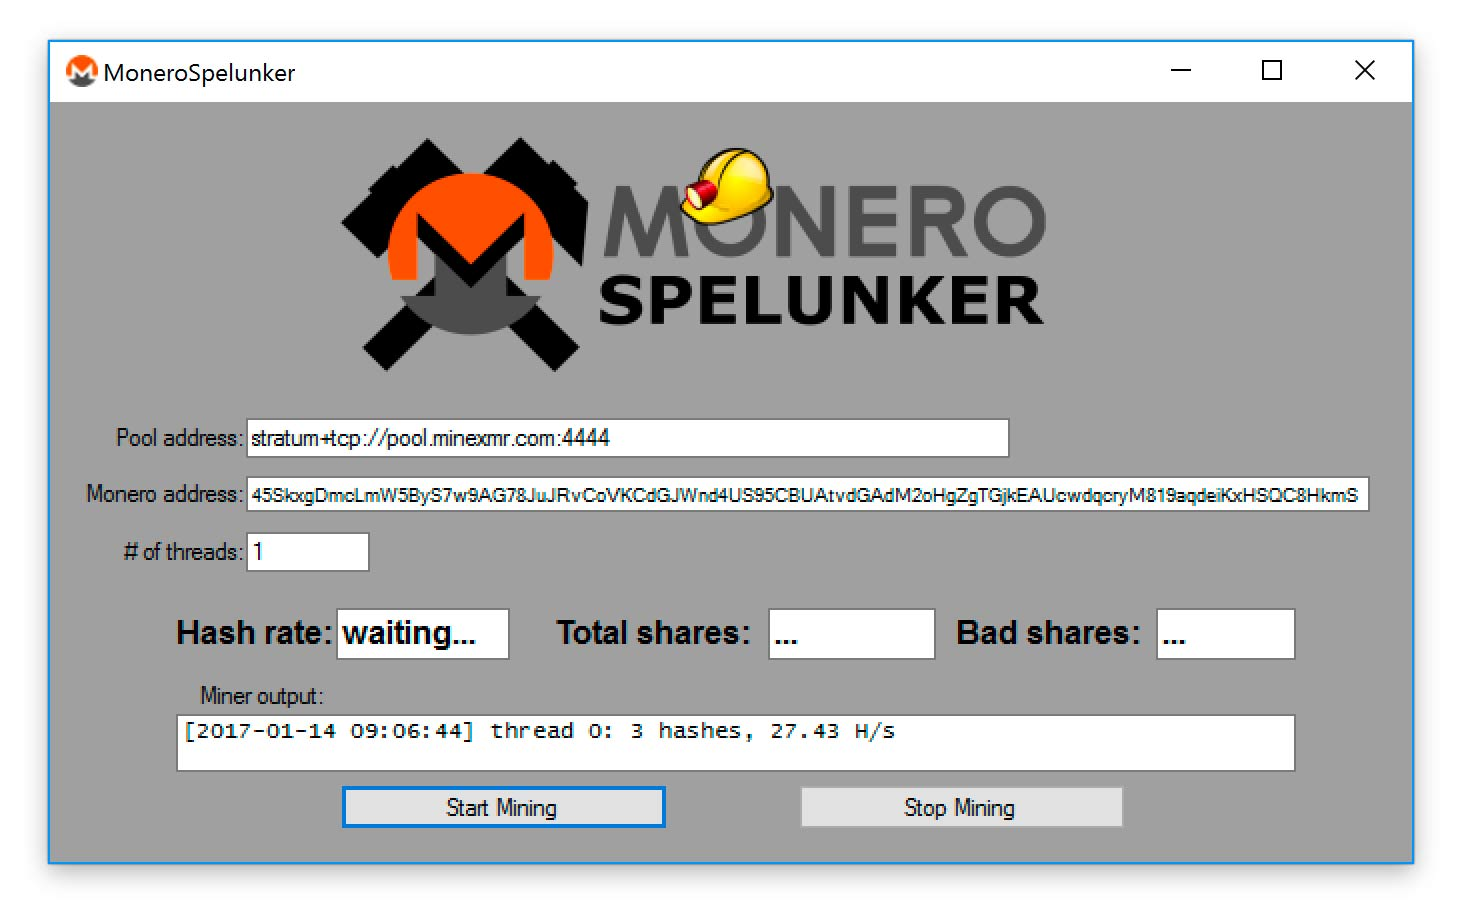
\includegraphics[width=0.8\linewidth]{./images/manual/spelunkerminer.jpg}
	\end{figure}
\subsubsection{Mining Monero on Fedora 24 and above}
Remember to replace \lstinline!WALLET_ADDRESS_HERE! with your own Monero wallet's public address. The ``-t 3'' option determines how many of your CPU threads will be used for mining. 
\begin{lstlisting}
yum -y install git curl-devel libcurl glib-devel libtool
git clone https://github.com/hyc/cpuminer-multi
cd cpuminer-multi
./autogen.sh
CFLAGS="-march=native" ./configure
make
sudo ./minerd -a cryptonight -o stratum+tcp://pool.minexmr.com:4444 -u WALLET_ADDRESS_HERE -p x -t 3
\end{lstlisting}
\subsubsection{Mining Monero on Ubuntu 14 and above}
	Remember to replace \lstinline!WALLET_ADDRESS_HERE! with your own Monero wallet's public address. The ``-t 3'' option determines how many of your CPU threads will be used for mining.
\begin{lstlisting}
sudo apt-get install git libcurl4-openssl-dev build-essential libjansson-dev autotools-dev automake
git clone https://github.com/hyc/cpuminer-multi
cd cpuminer-multi
./autogen.sh
CFLAGS="-march=native" ./configure
make
sudo ./minerd -a cryptonight -o stratum+tcp://pool.minexmr.com:4444 -u WALLET_ADDRESS_HERE -p x -t 3
\end{lstlisting}
\subsubsection{Checking your mining earnings}
	\begin{figure}[htbp!]
		\centering
		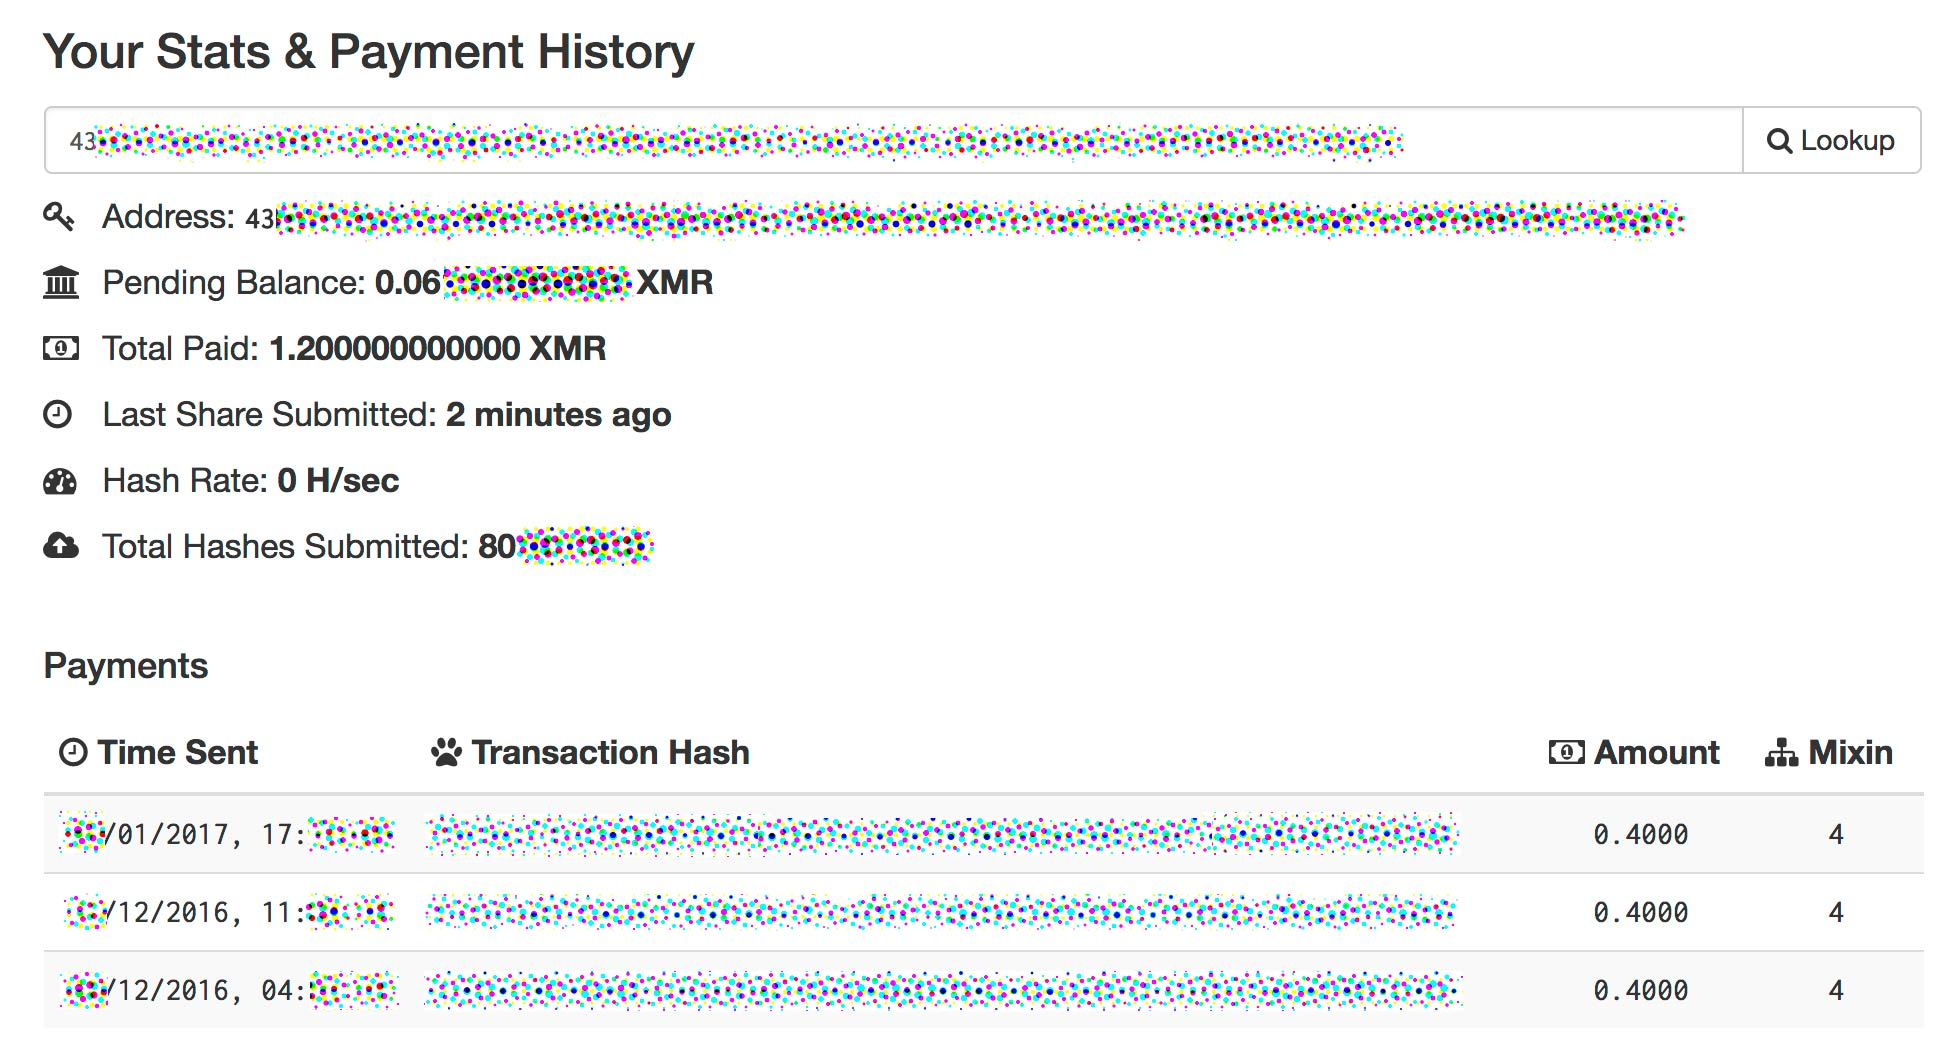
\includegraphics[width=0.8\linewidth]{./images/manual/mining-payments.jpg}
	\end{figure}
	To check how much Monero you have earned through your mining efforts, enter your wallet address into the ``Lookup'' box at the mining pool site. It will tell you how much you have earned, and how much has been paid out so far. \par
	Note that each mining pool has a payment threshold, which saves on transaction fees by only paying out once you have mined a certain amount of Monero. Be prepared for it to take days or weeks to receive your first payment, depending on the speed of your computer hardware. \par
	Note that with some pools, your Hash Rate will be reported as zero for most of the time, until you suddenly submit a 'share' to the pool from your mining efforts. You will temporarily see your Hash Rate reported, after which it will return to zero. This is normal for some pools, and you do not need to worry that something is not working correctly. As long as after a while you see the ``total hashes submitted'' figure increase, then your mining setup is working.


\section{Glossary of the most important Monero terms}
		Cite from \url{https://www.monero.how/monero-glossary}.
	\begin{itemize}
		\item Balance/Unlocked balance
		\item CLI/Command line interface
		\item Daemon
		\item Exchange
		\item GUI
		\item Integrated payment address
		\item Mining/Blocks/Blockchain
		\item Mining pool
		\item Payment id
		\item Privacy level/mixin
		\item Private key/Seed
		\item Public address
		\item Refresh/synchronization
		\item Stealth address
		\item Sweep unmixable
		\item Transaction priority
		\item View key
		\item Wallet/wallet files/wallet software
		\item XMR
	\end{itemize}
\subsubsection{Public address}
	Also known as your address or wallet address . An example address looks like this:\\ 
	\lstinline!43EH3omZSUYCmJYskCUx2tV5oB5tLVrp58AeMYLrFhcz2umUVQHiHu62nG5CS3mvcfgKHC3fPtq6DHkEbMjqvCAZJW5nw9E!
\subsubsection{Payment id}
	When someone sends you funds, they can specify a payment ID of their or your choice. Because Monero's privacy protections usually prevent you from knowing the source of funds that you receive, the payment ID can be used by the sender to identify themselves to you.
\subsubsection{Integrated payment address}
	To make it easier for other people to send you funds with a payment ID that you require, you can generate an integrated address to send to them which contains both your public address and the payment ID you request them to use.
\subsubsection{Wallet/wallet files/wallet software}
	Your wallet holds your private key, which allows you to view your funds and spend them. A wallet may be configued to only hold a view key, so that the wallet can observe your funds but not spend them. Your wallet also contains a list of transaction IDs and transaction keys, which allow you to see a list of payments you've previously made. \par
	If you create another wallet from your seed (which is a representation of your private key), then you will have the full ability to spend your funds but you will not be able to see a list of transactions that you've previously made. This is why, if you need to see a history of your transactions, that you should back up your wallet files and not just your seed. \par
	`Wallet' may refer to just the wallet files on your computer, or additionally to the wallet software that you run which allows you to view your wallet files and transact. Your wallet communicates with a Monero daemon to scan the blockchain for incoming transactions and to send new transactions.
\subsubsection{Private key/Seed}
	Your private key is what allows you to spend your funds. Your `seed' is just a 25 word representation of your private key which is easy for you to write down on paper. You must keep your private key a secret, or other people will be able to spend your funds. Your private key is the only thing you need to access and spend your funds. Your public address can be recovered from your private key, so you do not need to additionally keep a note of your public address.
\subsubsection{View key, also known as a secret view key or private view key}
	Your view key is normally kept private. If you wish, you can give out your view key so that others can observe the contents of your wallet. For security reasons, you may use your own view key to observe your funds on a computer which may be at risk of attack. Therefore if that computer became compromised, the attacker could see that you have funds, but not be able to steal them. Your private key would be kept safe and only used when you need to send funds when on a more secure computer.
\subsubsection{Daemon}
`Daemon' is a technical term for a program that runs in the background. Monero uses a daemon to synchronize with the Monero network to scan for incoming transactions and to send new transactions. Your wallet needs to use the daemon to scan the entire blockchain for incoming transactions, because only your wallet has your private view key. Only your private view key can be used to detect which transactions on the Monero network have been sent to you. This is a key part of Monero's privacy technology.
\subsubsection{Balance/Unlocked balance}
When someone sends you funds, they will appear in your balance. Once the Monero network has `confirmed' the transaction 10 times, which will take on average 20 minutes, your funds will become spendable and will be listed as part of your `unlocked' balance. The 10 confirmation minimum is necessary to prevent double spending by the sender.
\subsubsection{Refresh/synchronization}
	Because of Monero's privacy mechanisms, your private view key needs to be used to scan the blockchain to detect transactions destined for you. This means that until your wallet software has scanned the entire blockchain, you will not see your funds appear in your wallet's balance.
\subsubsection{Mining/Blocks/Blockchain}
Mining is the process by which the network of Monero nodes collectively verifies transactions, in exchange for a small transaction fee. When transactions are mined, this causes them to appear in a block, which is added to the blockchain. The blockchain is therefore the entire record of all Monero transactions that have ever taken place. Monero's privacy mechanisms ensure that the blockchain can only be used to reveal information about transactions to those involved in the transaction. The blockchain is necessary to prevent the double-spending of funds, because it contains the information necessary to verify that funds have not already been spent by their owner.
\subsubsection{Mining pool}
	A group of computers that together run mining software to process Monero transactions and collectively share in the reward. The advantage of a Mining pool is that a single computer would take too long to mine a single block if it were working alone, and so the owner of the computer would have to wait unreasonably long to receive their first share of the mining rewards.
\subsubsection{Privacy level/mixin}
When you send funds, Monero's privacy mechanism will obscure your funds as a possible source by `mixing in' other sources of funds in the transaction. It is impossible for any observer to know which is the real source of the funds, and only you can prove that you were the real source by deciding to reveal the secret transaction key generated by you for that transaction. \par
A mixin level of 4, which is the minimum allowable in the Monero GUI, will mean that your funds will appear to be one of 5 possible sources of funds for the transaction. In the GUI, the mixin level is referred to as the `privacy level'. Remember that every other person that sends a transaction may randomly select your funds to be a plausible source in their own transaction. This means that although it may at first seem like you are one of 5 possible senders, the aggregate effect of all Monero users constantly mixing each others' funds means your privacy level is radically higher than the number `5' would at first suggest. Over time, it will appear as if you've at some point plausibly directly or indirectly participated in transactions with most other Monero users, even if you're hardly ever using Monero.
\subsubsection{Transaction priority}
	Your transaction will be mined into a new block on the blockchain. However, if there are a lot of transactions occurring, your transaction may not make it into the very next block that is mined, and so you may have to wait a few more minutes for your transaction to be included in the blockchain. You can increase your transaction priority to compete for position in the next block that gets mined. Usually, there is no reason to increase your transaction priority because there will most often be room in the next block for your transaction. Monero has been designed to automatically increase the size of blocks as transaction volume increases, which means you only need to adjust your transaction priority higher if the Monero network is temporarily experiencing a surge in transaction volume and the Monero network has not yet adjusted upwards the sizes of blocks that are created to store those transactions.
\subsubsection{Sweep unmixable}
	A button that appears in the beta version of the Monero GUI that you don't have to worry about. It's only for those that received payments long ago, before RingCT and before denominations were used as part of Monero transactions.
\subsubsection{Exchange}
	A place you can go to exchange dollars, Bitcoin or other currencies for Monero.
\subsubsection{XMR}
The currency code for Monero.
\subsubsection{GUI}
	GUI Stands for Graphical User Interface. It makes it easy for you to use Monero.
\subsubsection{CLI/Command line interface}
	A text only application that does not have a graphical interface.
\subsubsection{Stealth address}
	When a transaction is sent, Monero does not publicly record the recipient's public address as the destination, and instead creates a new anonymous one-time address as the destination that is not linked to the recipient's public address. This one-time address is called a stealth address, because it ensures that your public address does not appear on the blockchain. Only the recipient has the necessary secret view key to scan the blockchain to locate these one-time destination addresses that contain the received funds.


\fi

\ifx\ProjectOff\undefined
\chapter{Monero Project}
\section{RPC Documentation}
	\subsection{Wallet}
The RPC interfaces are documented according to their namespaces as follows.
\subsubsection{wallet\_rpc\_server}
\begin{table}[!htbp]
	\centering
	\caption{The JSON RPC and their corresponding callbacks for wallet}
	\begin{tabular}{cc}
		\hline
		JSON RPC & Callback \\
		\hline
		\code{make_integrated_address} & \code{on_make_integrated_address} \\
		\hline
	\end{tabular}
\end{table}

\section{API}
	Every column of the key matrix will consist of keys from a single person in this part.
\subsubsection{proveRctMG}\label{proveRctMG}
	\begin{description}
		\item[Input]  
			\begin{itemize}
				\item \(msg\): message to sign
				\item \(\mathbf{inPk}=\Big[(pk_{j,i},c_{j,i})\Big]_{m\times n}\): input public key matrix of \(m\) rows and \(n\) columns
				\item \(\mathbf{inSk}=\left((sk_1,x_1^c),\dots,(sk_j,x_j^c),\dots,(sk_m,x_m^c)\right)\): input secret key vector of size \(m\)
				\item \(\mathbf{outSk}=(y_1,\dots,y_k,\dots,y_{m'})\): output secret key vector of size \(m'\)
				\item \(\mathbf{outPk}=\left((\hat{pk}_1,\hat{c}_1),\dots,(\hat{pk}_k,\hat{c}_k),\dots,(\hat{pk}_{m'},\hat{c}_{m'})\right)\): output public key vector of size \(m'\)
				\item \(\pi\): the column index of public key matrix corresponds to the secret key vector \(\mathbf{inSk}\)
				\item \(bH\): i.e. key for transaction fee of amount \(b\) is the paper
			\end{itemize}
		\item[Ouput] the multi-layer ring signature of the input message \(msg\)
		\item[Procedure]
			\begin{enumerate}
				\item for \(i=1,\dots,(m+1)\), \(sk_i^*=0\), where \(sk^*\) is a vector of key
				\item initialize a key matrix as 
					\[
						\mathbf{M}=\begin{bmatrix}
							I_1 &\dots &I_1 \\
							\vdots &\vdots &\vdots \\
							I_j &\dots &I_j \\
							\vdots &\vdots &\vdots \\
							I_{m+1} &\dots &I_{m+1}
						\end{bmatrix}_{(m+1)\times n}
					\]
					where vector \(I=(1,0,0,\dots,0)\) of length 32 is a key corresponding to the zero elliptic curve point
				\item update \(\mathbf{M}\) as  
					\[
						\mathbf{M}=\begin{bmatrix}
							pk_{1,1} &\dots &pk_{1,i} &\dots &pk_{1,n} \\
							 \vdots &\vdots &\vdots &\vdots &\vdots &\\
							pk_{j,1} &\dots &pk_{j,i} &\dots &pk_{j,n} \\
							 \vdots &\vdots &\vdots &\vdots &\vdots &\\
							pk_{m,1} &\dots &pk_{m,i} &\dots &pk_{m,n} \\
							\sum_{j=1}^{m}c_{j,1} &\dots &\sum_{j=1}^{m}c_{j,i} &\dots &\sum_{j=1}^{m}c_{j,n}
						\end{bmatrix}_{(m+1)\times n}
					\]
				\item update \(sk^*=(sk_1,\dots,sk_j,\dots,sk_m,\sum_{j=1}^m sk_j)\)
				\item update \(\mathbf{M}\) as  
					\[
						\mathbf{M}=\begin{bmatrix}
							pk_{1,1} &\dots &pk_{1,i} &\dots &pk_{1,n} \\
							 \vdots &\vdots &\vdots &\vdots &\vdots &\\
							pk_{j,1} &\dots &pk_{j,i} &\dots &pk_{j,n} \\
							 \vdots &\vdots &\vdots &\vdots &\vdots &\\
							pk_{m,1} &\dots &pk_{m,i} &\dots &pk_{m,n} \\
							\dots &\dots &\sum_{j=1}^{m}c_{j,1}-\sum_{k=1}^{m'}\hat{c}_k-bH  &\dots &\sum_{j=1}^{m}c_{j,n}-\sum_{k=1}^{m'}\hat{c}_k-bH 
						\end{bmatrix}_{(m+1)\times n}
					\]
				\item update \(sk^*=(sk_1,\dots,sk_j,\dots,sk_m,\sum_{j=1}^m sk_j-\sum_{k=1}^{m'}y_k)\)
				\item hand over \(msg\), \(\mathbf{M}\), \(sk^*\), \(\pi\) and \(m\) to function \texttt{MLSAG\_Gen}, (i.e., treat all public keys but the last as double-spendable) and return the signature by \texttt{MLSAG\_Gen}
			\end{enumerate}
	\end{description}
\subsubsection{proveRctMGSimple} 
	\begin{description}
		\item[Input]
			\begin{itemize}
				\item \(msg\): message to sign
				\item \(inPK=\left((pk_1,c_1),(pk_2,c_2),\dots,(pk_m,c_m)\right)\): input public key vector of length \(n\), where \(pk_i\) is the public key, and \(c_i\) is the commitment
				\item \(inSK=(sk,x^c)\): input secret key, where \(sk\) is the actual secret key, and \(x^c\) is the mask key
				\item \(y\): output secret key, i.e. the mask value
				\item \(\hat{c}\): output public key, i.e., the output commitment
				\item \(\pi\): index of the public key in \(inPK\) paired with \(inSK\)
			\end{itemize}
		\item[Ouput] the simple(one-layer) ring signature of the input message \(msg\)
		\item[Procedure]
			\begin{enumerate}
				\item initialize \(\mathbf{M}=[ ]_{2\times n}\), a \(2\times n\) matrix
				\item update 
					\[
						\mathbf{M}=
						\begin{bmatrix}
							\dots &pk_i &\dots \\
							\dots &c_i &\dots
						\end{bmatrix}
					\]
					and then
					\[
						\mathbf{M}=
						\begin{bmatrix}
							\dots &pk_i &\dots \\
							\dots &c_i-\hat{c} &\dots
						\end{bmatrix}
					\]
				\item estimate \(sk^*=(sk,sk-y)\)
				\item hand over \(msg\), \(\mathbf{M}\), \(sk^*\), \(\pi\) and \(1\) to function \texttt{MLSAG\_Gen}, (i.e., treat all public keys but the last as double-spendable) and return the signature by \texttt{MLSAG\_Gen}
			\end{enumerate}
	\end{description}
\subsubsection{MLSAG\_Gen} 
	\begin{description}
		\item[Input]
			\begin{itemize}
				\item \(msg\): message to sign
				\item \(\mathbf{Y}=\Big[y_{j,i}\Big]_{m\times n}\): the public key matrix of \(m\) rows and \(n\) columns
				\item \(\mathbf{x}=(x_1,x_2,\dots,x_m)\): the secret key vector of length \(m\) from the singer 
				\item \(\pi\): the column index of public key matrix corresponds to the secret key vector \(\mathbf{x}\)
				\item \(m'\): the number of double spendable rows, should satisfy \(m'<m\)
			\end{itemize}
		\item[Output] signature as \( (I_1,\dots,I_m,c_1,\mathbf{S}=[s_{j,i}]_{m\times n})\) where \(I_j\) is the key image, \(c_1\) is the first hash (treated as a scalar) in the ring, and \(\mathbf{S}\) is the scalar matrix of randomly generated to make up the ring. (c.f.g struct \texttt{mgSig} in the \texttt{rctTypes.h})
		\item[Procedure]
			\begin{enumerate}
				\item for \(j\leftarrow 1,\dots,m'\), generate \(\alpha_j\) randomly and estimate 
					\begin{itemize}
						\item \(L_j\leftarrow\alpha_i G\)
						\item \(H_{P_j}\leftarrow hashToPoint(Y_{j,\pi})\)
						\item \(R_j \leftarrow \alpha_j H_{P_j}\)
						\item \(I_j\leftarrow x_j H_{P_j}\)
					\end{itemize}
				\item for \(j\leftarrow(m'+1),\dots,m\), generate \(\alpha_j\) randomly and estimate \(L_j\leftarrow\alpha_i G\)
				\item calculate \(c_{old}\leftarrow H(msg,Y_{1,\pi},L_j,R_j,\dots,Y_{m',\pi},L_{m'},R_{m'},Y_{(m'+1),\pi},L_{(m'+1)},\dots,Y_{m,\pi},L_{m})\)
				\item initialize \(i\leftarrow(\pi+1)\bmod n\), if \(i=0\), set \(c_1\leftarrow c_{old}\)
				\item for \(i\leftarrow(\pi+1),\dots,n,1,\dots,(\pi-1)\)
					\begin{enumerate}
						\item generate \(s_{j,i}\) randomly for \(j\leftarrow1,\dots,m\)
						\item for \(j\leftarrow1,\dots,m'\), calculate
							\begin{itemize}
								\item \(L_j\leftarrow s_{j,i} G+c_{old} Y_{j,i}\)
								\item \(R_j \leftarrow s_{j,i} hashToPoint(Y_{j,i}) + c_{old} I_{j}\)
							\end{itemize}
						\item for \(j\leftarrow(m'+1),\dots,m\), estimate \(L_j\leftarrow s_{j,i} G+c_{old} Y_{j,i}\)
						\item update \(c\leftarrow H(msg,Y_{1,i},L_j,R_j,\dots,Y_{m',i},L_{m'},R_{m'},\dots,Y_{(m'+1),i},L_{(m'+1)},\dots,Y_{m,i},L_{m})\)
						\item increment \(i\leftarrow(i+1)\bmod n\), if \(i=0\), set \(c_1\leftarrow c_{old}\)
						\item update \(c_{old}\leftarrow c\)
					\end{enumerate}
				\item update \(s_{j,\pi}\leftarrow\alpha_j-c x_j\)
			\end{enumerate}
	\end{description}
\subsubsection{construct\_tx\_and\_get\_tx\_key} 
	\begin{description}
		\item[Input]
			\begin{itemize}
				\item \(\mathbf{ack}\): account key of the payer, consisting of two seckey-pubkey pairs as \( (a,A=a\cdot G)\) for viewing and \( (b,B=b\cdot G)\) for spending
				\item \(\mathbf{inCoin}=\{inCoin_i=(amt_i,\{(P_{i,j},C_{i,j},o_{i,j})\}_{j=1}^{l_i},R_i,k_i,k_i')\}_{i=1}^m\): input coin ring vector, where for each \(inCoin_i\)
					\begin{itemize}
						\item \(amt_i\) is the amount of the real input coin
						\item \(P_{i,j}\) is the one-time address of the j-th coin
						\item \(C_{i,j}\) is the commitment of amount of the j-th coin
						\item \(o_{i,j}\) is the global output index of the j-th coin
						\item \(R_i\) is the key for the tx producing the real input coin
						\item \(k_i\) is the index of the real input coin
						\item \(k_i'\) is the index of the real input coin in the tx containing it
					\end{itemize}
				\item \(\mathbf{outDest}=\{(\hat{amt}_j,A_j,B_j)\}\): output destination vector, where for the j-th destination, \(\hat{amt}_j\) is the amount to send, \(A_j\) is the public key for viewing, and \(B_j\) is the public key for spending
					\item \(extra\): extra field storing payment ID, public tx key, etc
			\end{itemize}
		\item[Output] 
			\begin{itemize}
				\item \(\mathbf{tx}\): the constructed tx with RCT signature set up
			\end{itemize}
		\item[Procedure]
			\begin{enumerate}
				\item generate a tx key pair \( (r,R=r\cdot G)\)
				\item remove pubkeys in \(extra\) if any and add \(R\) to \(extra\)
				\item encrypt the stealth payment ID if any in \(extra\) with \(r\cdot A\)
				\item For each \(inCoin_i\),
					\begin{itemize}
						\item derive the address key pair \( (x_i^*,P_i^*)=(H_s(a\cdot R_i||k_i')+b, H_s(a\cdot R_i||k_i')\cdot G+B)\) and key image \(I_i=x_i^*\cdot H_p(P_i^*)\)
						\item ensure if \(P_i^*\) is equal to the one \(P_{i,k_1}\) specified in \(inCoin_i\)
						\item make an input entry as \( inToKey_i=(amt_i^*,I_i,\{o_{i,1}^*=o_{i,1},o_{i,2}^*=o_{i,2}-o_{i,1},\dots,o_{i,j}^*=o_{i,j}-o_{i,j-1},\dots\}\)
					\end{itemize}
				\item sort \(outDest_i\in\mathbf{outDest}\) in ascending order of their amount
				\item For each \(outDest_j\), 
					\begin{itemize}
						\item compute the amount key \(amtKey_j=H_s(r\cdot A_j||j)\)
						\item calculate the one-time key \(\hat{P}_j=amtKey_j\cdot G+B_j\)
						\item make an output coin as \(outCoin_j=(\hat{amt}_j,\hat{P}_j)\)
					\end{itemize}
				\item assert \(\sum amt_i>\sum\hat{amt}_j\)
				\item If the number \(m>1\) of input coin ring, use simple RCT, or else use the full one
					\begin{itemize}
						\item For simple RCT,
							\begin{enumerate}
								\item \(\bM=[]_{1\times m}\)
								\item compute the real input amount key and commitment \(\{(x_i,C_i)\}_{i=1}^m\)
								\item update the i-th column of \(\bM\) as \(M_i=[(P_{i,j},C_{i,j})]_{j=1}^{l_i}\)
								\item save a copy \(\{amt_i^*\}\) of input amount \(\{amt_i\}\)
								\item save a copy \(\{\hat{amt}_j^*\}\) of output amount \(\{\hat{amt}_j\}\)
								\item mask the amount in inputs \(inToKey_i\) and outputs \(outCoin_j\) by zeroing them
								\item compute the hash \(h_{pre}\) of the tx prefix including the version, unlock time, \(\{inToKey_i\}\), \(\{outCoin_j\}\) and extra nonces
								\item  delegate the signing job to \code{rct::genRctSimple} with message \(h_{pre}\), input secret key vector \(\{(x_i,C_i)\}\), destination \(\{outCoin_j\}\), input amount \(\{amt_i^*\}\), output amount vector \(\{\hat{amt}_j^*\}\), tx fee (\(\sum amt_i^*-\sum \hat{amt}_j^*\)), mix-in matrix \(\bM\), amount key vector \(\{amtKey_i\}\), real input index \(\{k_i\}\) and get back mask values and MLSAG
							\end{enumerate}
						\item For non-simple RCT,
							\begin{enumerate}
								\item \(\bM=[]_{1\times l_1}\)
								\item \(\bM=[(P_{1,i},C_{1,i})]_{1\times l_1}\)
								\item save a copy \(\{amt_i^*\}\) of input amount \(\{amt_i\}\)
								\item save a copy \(\{\hat{amt}_j^*\}\) of output amount \(\{\hat{amt}_j\}\)
								\item append tx fee (\(amt_1^*-\sum \hat{amt}_j^*\)) to \(\{\hat{amt}_j^*\}\)
								\item mask the amount in inputs \(inToKey_i\) and outputs \(outCoin_j\) by zeroing them
								\item compute the hash \(h_{pre}\) of the tx prefix including the version, unlock time, \(\{inToKey_i\}\), \(\{outCoin_j\}\) and extra nonces
								\item  delegate the signing job to \code{rct::genRct} with message \(h_{pre}\), input secret key vector \((x_1,C_1)\), destination \(\{outCoin_j\}\), output amount vector \(\{\hat{amt}_j^*\}\), mix-in matrix \(\bM\), amount key vector \(\{amtKey_i\}\), real input index \(k_1\) and get back mask values and MLSAG
							\end{enumerate}
					\end{itemize}
			\end{enumerate}
	\end{description}
\subsubsection{ } 
	\begin{description}
		\item[Input]
			\begin{itemize}
				\item 
			\end{itemize}
		\item[Output]
		\item[Procedure]
			\begin{enumerate}
				\item 
			\end{enumerate}
	\end{description}

\fi

\ifx\ExperimentOff
\chapter{Experiment On RingCT}
	\section{Overview}
To evaluate the effectiveness of the proposed RingCT+ scheme, two criteria of interest are the time complexity of signature generation and latency from network transmission under different circumstances. To compare our RingCT+ and the original RingCT in current Monero, we will estimate the aforementioned criteria under two circumstances, i.e., the same size/number of mixins and the same size of anomynity set. And the detailed methods go as follow. (For convience, the original RingCT in Monero will be simply called RingCT).
\section{Parameters}
	\begin{itemize}
		\item \(l\): the size of a single ring in the mixin matrix (The range of \(l\) to choose is TBD)
		\item \(m\): the number of real input coins to mix (The range of \(l\) to choose is TBD)
		\item \(N\): number of tests on each \( (l,m)\) pair
	\end{itemize}
	Given \(l\) and \(m\), the size of mixins \(S_m\) and the size of the anomynity set \(S_a\) of the RingCT and our RingCT+ can be derived as table
	\begin{table}[!htbp]
		\centering
		\begin{tabular}{ccc}
			\hline
			Schemes & \(S_m\) & \(S_a\) \\
			\hline
			RingCT & \((l-1)\cdot m\) & \(l\) \\
			RingCT+ & \( (l-1)\cdot m\) & \(l^m\) \\
			\hline
		\end{tabular}
	\end{table}
\section{The time complexity of signature generation}
To get rid of the possible influence by other factors, tests to evaluate the time complexity focus on the core function \code{proveRctMG} which is responbile of building the mixin matrix step by step and then calculate the signature based on the resultant mix-in matrix. And for brevity, let's denote the counterpart of function \code{proveRctMG} in the monero project, as \code{proveRctMG2}.
\subsection{Methodology}
	\begin{enumerate}
		\item For each \( (l,m)\) to check, we generate an l-by-m valid public key matrix \(M= [pk_{i,j}]_{l\times m}\) randomly in such a way that all the \(m\) keys in the 1st row are generated with a associated secret key. That's, they are treated as addresses for real input coins.
		\item To evaulate the RingCT signature function, we pass \(M\) and adapt other relevant parameters accordingly to \code{proveRctMG}, and record the time of execution for signing based on these \(M\).
		\item To evaulate the RingCT+ signature function, we pass \(M\) and adapt other relevant parameters accordingly to \code{proveRctMG2}, and record the time of execution for signing based on these \(M\).
		\item Repeat the above process on the same \( (l,m)\) for \(N\) times, and calculate the average time for these \(N\) test cases.
		\item Repeat the above process on other \( (l,m)\) for \(N\) times.
	\end{enumerate}
	By the comparison of the average time for signing under RingCT and RingCT+, put forward the corresponding conclusion. For example, how much overhead stems from the RingCT+.
\section{The latency due to network transmission}
Similarly, tests to estimate latency are conducted subject to the core RPC calls from wallets from daemons.\par
And here parameters are a little different. To achieve the same size of anomynity set (say \(S_a=l^m\)) for \(m\) input coins, the size of a single ring in the RingCT+ would be only \(l\), while it's \(l^m\) for the RingCT. Hence, the dimension of the public key matrix will need to be adjust accordingly as shown in the following methodology part.
\subsection{Methodology}
	\begin{enumerate}
		\item For each \( (l^m,m)\) to check, we generate randomly an l-by-m valid public key matrix \(M_1= [pk_{i,j}]_{l\times m}\) and an \(l^m\)-by-m one \(M_2=[pk_{i,j}]_{l^m\times m}\), in such a way that all the \(m\) keys in the 1st row of both \(M_1\) and \(M_2\) are generated with a associated secret key. That's, they are treated as addresses for real input coins.
		\item Generate signatures for the RingCT and RingCT+ by function \code{proveRctMG} on \(M_1\) and \code{proveRctMG2} on \(M_2\) respectively, and collect the output signature as \(Sig_1\) and \(Sig_2\).
		\item For each \(Sig_i\) (\(i\in {1,2}\)), transfer the signed transaction bound with \(Sig_i\) to a preset standalone daemon, and record the time from the beginning of the transfer and the ending of receving (or parsing?) on the daemon side.
		\item Repeat the above process on the same \( (l^m,m)\) for \(N\) times, and calculate the average time for these \(N\) test cases.
		\item Repeat the above process on other \( (l^m,m)\) for \(N\) times.
	\end{enumerate}
	By the comparison of the average time for transmisson under RingCT and RingCT+, put forward the corresponding conclusion. For example, how much latency has been reduced due to optimised anomynity provided by RingCT+.

\fi

\ifx\BlogSeriesOff\undefined
\chapter{Blog Series about XMR}
\section{Interesting Sites}
	\begin{itemize}
		\item \url{https://moneroeric.com/monero-sites/}
		\item \url{https://monero.stackexchange.com/}
	\end{itemize}
\section{Understanding Monero Cryptography, Privacy -- Introduction}
	\textbf{Cited from} \href{https://steemit.com/monero/@luigi1111/understanding-monero-cryptography-privacy-introduction}{XMR crypto blog series} by \href{https://github.com/luigi1111}{luigi1111}.\par

\begin{displayquote}
This is part two of a series of unknown size; it'll be done when it's done. Part one is \href{https://steemit.com/monero/@luigi1111/understanding-monero-cryptography-privacy-introduction}{here}.\\\\
Part one focuses on the basics: ECC, the particular curve, private and public "keys", and a bonus section on how Monero addresses are generated. \\\\
Note: Monero is based on the \href{https://cryptonote.org/whitepaper.pdf}{Cryptonote protocol} -- though it has diverged and will continue to diverge -- along with numerous other coins; much of this series applies equally well to the others with some caveats. Monero is easily the largest and most active Cryptonote-based project.
\end{displayquote}

Hello! I'm an autodidact enthusiast of cryptography, particularly in relation to the crypto-currency \href{https://getmonero.org/}{Monero}. Naturally, you should not assume everything I say is correct, and I hope any egregious errors are pointed out so I can fix them (and help my own understanding). Just calling me an idiot is fine too.

\begin{figure}[H]
	\centering
	
\includegraphics[width=0.4\linewidth]{./images/blog-series/xmr-crypto-luigi1111/idiot-doctor.jpg}
\end{figure}

Monero's tagline is ``Secure, Private, Untraceable.'' Secure could refer to a number of facets of a crypto-currency, but here we are only particularly interested in security relating to privacy/anonymity. These articles will be looking at how Monero achieves ``privacy'', that is unlinkability and untraceability, with references to security where appropriate. This article focuses on some concepts, which will hopefully make understanding the others easier. Without further ado, let's get into it!

\subsection{What is Elliptic Curve Cryptography?}
Alright, so what is ECC? From \href{https://en.wikipedia.org/wiki/Elliptic_curve_cryptography}{Wikipedia}: ``\textbf{Elliptic curve cryptography (ECC)} is an approach to \href{https://en.wikipedia.org/wiki/Public-key_cryptography}{public-key cryptography} based on the \href{https://en.wikipedia.org/wiki/Algebraic_structure}{algebraic structure} of \href{https://en.wikipedia.org/wiki/Elliptic_curve}{elliptic curves} over \href{https://en.wikipedia.org/wiki/Finite_field}{finite fields}.''

Now, what does that mean? \emph{I have no idea.}

More seriously, let's go through it:
	\begin{enumerate}
		\item Public-Key Cryptography, or asymmetric cryptography, uses a pair of keys instead of a single private key as in symmetric cryptography (e.g., \href{https://en.wikipedia.org/wiki/Advanced_Encryption_Standard}{AES}): a public key, to be given out to "the world"; and a private key, to be always kept secret. To be secure, it must be hard intractable to figure out the private key given the public key; to be usable it must be easy to calculate the public key given the private key. ECC relies on the \href{https://en.wikipedia.org/wiki/Discrete_logarithm}{ECDLP} for its security. \textbf{Takeaways: public/private key pair; private->public is easy, but public->private is "impossible".}
		\item ``algebraic structure of elliptic curves'': \emph{What is this???} It is a plane curve satisfying \(y^2=x^3+ax+b\). It might look something like \figurename~\ref{fig-xmr-crypto-luigi1111-elliptic-curve-eg}\\
			\emph{Who cares?} Right, probably no one. In case someone does, there's a wealth of articles (many related to Bitcoin) out there that explain in detail how they work, how addition is possible, etc. Some examples: \href{http://andrea.corbellini.name/2015/05/17/elliptic-curve-cryptography-a-gentle-introduction/}{A, B, C (a series itself)}. Numerous videos are out there too, if you're into that. \textbf{Takeaways: none, this funny-looking curve will not help you understand and isn't even how Monero's curve looks.}
		\item ``over finite fields'': this just means curve points are taken modulo some (large, prime) number. Everyone is familiar with modular addition and subtraction at least (even if they've never heard the word) due to our time-keeping. \emph{If it is 10am, what time will it be in 5 hours?} \textbf{Congrats, you just did modular addition.} An elliptic curve over a finite field might look something like \figurename~\ref{fig-xmr-crypto-luigi1111-elliptic-curve-GF-eg}\\
			\textit{Whoa, that looks odd.} Yes, it does. \textbf{Takeaways: none. Actually, note how the points are ``reflected'' over an invisible line in the center.}
	\end{enumerate}
\begin{figure}[H]
	\begin{subfigure}{0.4\linewidth}
		\centering
		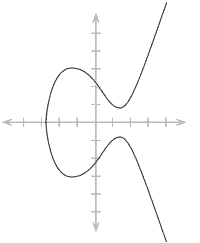
\includegraphics[width=0.6\linewidth]{./images/blog-series/xmr-crypto-luigi1111/elliptic-curve-eg.png}
		\caption{An example of elliptic curves}\label{fig-xmr-crypto-luigi1111-elliptic-curve-eg}
	\end{subfigure}
	\begin{subfigure}{0.55\linewidth}
		\centering
		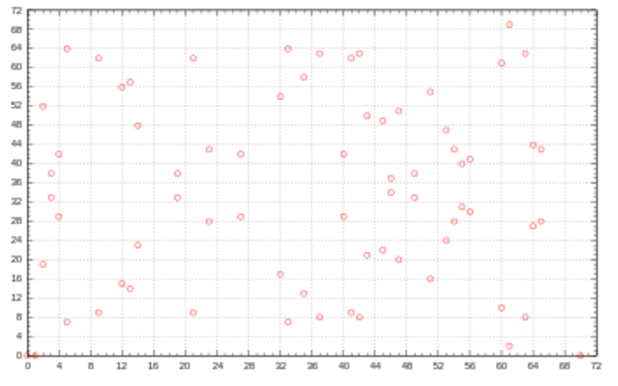
\includegraphics[width=0.8\linewidth]{./images/blog-series/xmr-crypto-luigi1111/elliptic-curve-GF-eg.png}
		\caption{An example of elliptic curves}\label{fig-xmr-crypto-luigi1111-elliptic-curve-GF-eg}
	\end{subfigure}
\end{figure}
A primary benefit of using ECC vs something like \href{https://en.wikipedia.org/wiki/RSA_(cryptosystem)}{RSA} is that keys are much smaller for similar security levels.

\subsubsection{I believe the only things you need to know to proceed are:}
	\begin{enumerate}
		\item A point on the curve can be added to or subtracted from another point, or itself.
		\item A point cannot be multiplied or divided by another point.
		\item Adding a point to itself allows ``scalar multiplication'', \textbf{which is where the magic happens}.
	\end{enumerate}

Subtracting a point from itself isn't very useful, as it'll just return the ECC equivalent of 0. Division by integer isn't possible (the equivalent modular operation -- modular multiplicative inverse -- is, but only with knowledge of the original scalar).

Scalar multiplication is just adding a point to itself over and over; given a point \(A\), \(5A = A + A + A + A + A\). Since we use astronomically large scalars to prevent easy brute-forcing, we use techniques like \href{https://en.wikipedia.org/wiki/Elliptic_curve_point_multiplication#Double-and-add}{double-and-add} to allow computation in near-logarithmic time (i.e., really fast!). A quick example:

Suppose our scalar is 27, and we want to compute \(27A\). Using the naive method, we'd need 26 additions. Instead:
	\begin{enumerate}
		\item Add \(A\) to itself: \(2A\). Let's call this new point B.
		\item Add \(B\) to itself: \(2B = 4A = C\).
		\item Add \(C\) to itself: \(2C = 4B = 8A = D\).
		\item Add \(D\) to itself: \(2D = 4C = 8B = 16A = E\).
		\item Add \(D\) to \(E\): \(24A = F\).
		\item Add \(B\) to \(F\): \(26A = G\).
		\item Add \(A\) to \(G: 27A\)
	\end{enumerate}

We went from 26 additions to 7. The difference grows exponentially with larger scalars. The speed difference for an average-size scalar is something along the lines of ``all the energy in the universe isn't enough'' and ``takes less than 1/100th of a second on an average computer'', which is interesting to ponder.

That's it for general ECC stuff! If you want more in-depth technical details, please see the links above. :)

\subsection{The Monero Curve and Private and Public ``Keys''}
Now, onto the Monero-specific stuff. Finally.

First some boring stuff like curve constants. From the \href{https://cryptonote.org/whitepaper.pdf}{Cryptonote whitepaper}, we get:
	\begin{itemize}
		\item \(q\): a prime number; \(q=2^{255}-19\)
		\item \(d\): an element of \(\mathbb{F}_q\); \(d=-121665/121666\)
		\item \(E\): an elliptic curve equation; \(-x^2+y^2=1+dx^2y^2\)
		\item \(G\): a base point; \(G=(x,-4/5)\)
		\item \(l\): a prime order of the base point; \(l=2^{252}+27742317777372353535851937790883648493\);
		\item \(H_s\): a cryptographic hash function \({0,1}^*\rightarrow \mathbb{F}_q\)
		\item \(H_p\): a deterministic hash function \(E(\mathbb{F})\rightarrow E(\mathbb{F}_q)\)
	\end{itemize}

We are dealing with the \href{https://en.wikipedia.org/wiki/EdDSA#Ed25519}{Ed25519} curve, which is a \href{https://en.wikipedia.org/wiki/Twisted_Edwards_curve}{Twisted Edwards Curve}. \emph{Good, more meaningless details!}

\textbf{Let's quickly go through it:}
\begin{itemize}
	\item \(q\): this is the total number of points on this curve. It is mostly irrelevant for our purposes.
	\item \(d\): an element used in the curve equation below. Not important.
	\item \(E\): the equation for our Ed25519 curve. \textit{Wow, shiny!} Not important.
	\item \(G\): the base point or generator point. \textbf{This is important!} It is the base from which many operations start. It is the ``A'' in the above example. In hex, which all of our keys are commonly represented in, it looks like: ``5866666666666666666666666666666666666666666666666666666666666666''. Great, back to useless information.
	\item \(l\): the ``order'' of the above base point. \textbf{This is important}, as it defines the maximum number of points we can use, and the maximum size our scalars can be. This number is like the number ``12'' to a clock; adding points or scalars together that would ``go over'' means they will ``wrap around'' instead. If you could add \(G\) to itself over and over and over until you reached l-1 number of additions, you would end up back at \(G\).
	\item \(H_s\) and \(H_p\): s means scalar, \(p\) means point. These will be discussed in a later article.
\end{itemize}

\textbf{Note:}
	\begin{enumerate}
		\item Scalars (private keys, really just large integers) are always represented by lowercase letters in equations.
		\item Points (public keys, really an encoded coordinate on the curve) are always represented by uppercase letters.
	\end{enumerate}
	In the ``real world'' (user-facing), both private and public keys in Monero are represented by 64 hex characters, similar to the above representation of \(G\). Time for more useless information. Scalars are straightforwardly represented as \href{https://en.wikipedia.org/wiki/Endianness#Little}{little-endian} integers (any integer between 0 and \(l\) is valid), while points are specially encoded in a way that is too complex for this article. \emph{Or maybe I haven't cared enough about the encoding to research it}.

	If we use \(x\) as our private key and P as our public key, then \(P = xG\).

Some ``fun'' examples:
	\begin{enumerate}
		\item \(x = 1\) or ``0100000000000000000000000000000000000000000000000000000000000000'' (remember little-endian); \(P\) = ``5866666666666666666666666666666666666666666666666666666666666666'' or \(G\). (\(1G = G\))
		\item \(x = l - 1\) or ``ecd3f55c1a631258d69cf7a2def9de1400000000000000000000000000000010''; \\\(P\) = ``58666666666666666666666666666666666666666666666666666666666666e6'' (note similarity to \(G\)); This is the last point before wrapping around. You can think of it like \(-G\). Adding \(G\) to this value will produce a special identity element, the same as multiplying a point by 0 or order \(l\), or subtracting a point from itself.
		\item The integer  \((l+1) / 2\), ``f7e97a2e8d31092c6bce7b51ef7c6f0a00000000000000000000000000000008'', produces the point farthest away from \(G\) (close enough, it and the next point are tied due to \(l\) being odd), ``ac1999070321b2c6309cc8e31aa89a8b3baa75b5f8febf47855555a3e744bcf0'', similar to how 6 is farthest away from 12 on a clock. It (just like \(G\) and \textbf{every} other point) has a complimentary point (in this case produced by \((l-1) / 2\)), with which it will sum to the identity element.
	\end{enumerate}
\subsection{Monero Accounts and Addresses}
This has gone a little long, so I'll just briefly restate the information available \href{https://xmr.llcoins.net/addresstests.html}{here} for the standard deterministic derivation. The reason we have two key pairs will be discussed in a future article on stealth addresses.
	\begin{enumerate}
		\item Choose a random private spend key, typically by creating 256 random bits then ``reducing'' mod \(l\). Call this key \(b\) (to match the whitepaper -- it's confusing I know).
		\item Hash \(b\) with the chosen algorithm, \(H\) (Keccak\_256 in our usage). Interpret the result as an integer and reduce it mod l as before. Call this key \(a\).
		\item Calculate \(B = bG\) and \(A = aG\). These are your public spend and public view keys.
		\item Hash (prefix (0x12 in standard Monero) + \(B\) + \(A\)) with \(H\).
		\item Append the first four bytes of the result to (prefix + \(B\) + \(A\)). This will be 69 bytes (1 + 32 + 32 + 4).
		\item Convert to cnBase58. This is not as straightforward as regular base58, as it uses blocks and padding to result in fixed-length conversions. 69 bytes will always be 95 cnBase58 characters.
	\end{enumerate}
	Integrated addresses (described \href{http://pastebin.com/bp5RKXuC}{here}) are the same as above, but with an 8 byte Payment ID appended to \(A\) in step 4 above and a different prefix (0x13).

	That does it for the introduction! Hopefully it wasn't completely incoherent rambling. Additional articles on stealth addresses and ring signatures will be coming out sometime soon. \textbf{Feedback is appreciated.}

\begin{figure}[H]
	\centering
	
\includegraphics[width=0.5\linewidth]{./images/blog-series/xmr-crypto-luigi1111/TLDR.jpg}
\end{figure}

For those of you looking for a TL;DR (or if you're just bored out of your mind), I've included a random picture (but no TL;DR).

\begin{figure}[H]
	\centering
	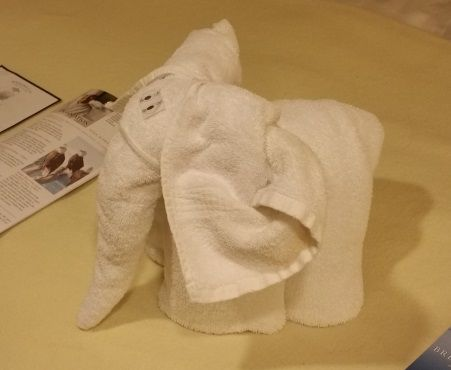
\includegraphics[width=0.5\linewidth]{./images/blog-series/xmr-crypto-luigi1111/rand-image.jpg}
\end{figure}

Until next time!


\section{Understanding Monero Cryptography, Privacy Part 2 -- Stealth Addresses}
	\textbf{Cited from} \href{https://steemit.com/monero/@luigi1111/understanding-monero-cryptography-privacy-part-2-stealth-addresses}{blog} by \href{https://github.com/luigi1111}{luigi1111}.\par
\begin{displayquote}
This is part two of a series of unknown size; it'll be done when it's done. Part one is \href{https://steemit.com/monero/@luigi1111/understanding-monero-cryptography-privacy-introduction}{here}.\\\\
Part two focuses on stealth addresses, an essential part of the protocol.\\\\
Note: Monero is based on the \href{https://cryptonote.org/whitepaper.pdf}{Cryptonote protocol} -- though it has diverged and will continue to diverge -- along with numerous other coins; much of this series applies equally well to the others with some caveats. Monero is easily the largest and most active Cryptonote-based project.
\end{displayquote}

Hello! I am back with part two of my series on Monero cryptography and privacy; in this series, I'm attempting to make the concepts as easy to understand as possible. I want you to have the same ``lightbulb'' moments I had when I first ``got'' these concepts (my understanding has evolved over a period of time).\par
In part two, we will be discussing stealth addresses, though you may learn some new concepts along the way. Stealth addresses are one of the two complementary techniques used to provide sender/receiver privacy in Monero.\par
So, what are stealth addresses? Well, they look like this:
\begin{figure}[H]
	\centering
	
\includegraphics[width=0.8\linewidth]{./images/blog-series/xmr-crypto-luigi1111/stealth-address-kidding.png}
\end{figure}
(just kidding)\par
In my own words, stealth addressing is a technique whereby a \textbf{sender} can take a \textbf{recipient's} public address and transform it to a one-time address such that:
\begin{enumerate}
	\item it is \textbf{publicly unlinkable} to the original public address;
	\item it is \textbf{publicly unlinkable} to \textbf{any} other one-time address;
	\item only the \textbf{recipient} can link all their payments together
	\item only the \textbf{recipient} can derive the secret key associated with the one-time address
\end{enumerate}
Using stealth addressing, a recipient can publish one address and receive unlimited* publicly unlinkable payments.\par

*[The chance of a \href{https://en.wikipedia.org/wiki/Collision_(computer_science)}{collision} (two stealth addresses being the same) is cryptographically negligible. Using the \href{https://en.wikipedia.org/wiki/Birthday_problem}{Birthday Paradox} we can roughly estimate it would take \(\sqrt{l}\), or about \(2^{126}\), stealth addresses being created before having a 50\% chance of a collision. The result would be that the colliding addresses become publicly linkable to each other, but not to any others. There is another, worse problem that would occur in Monero if two stealth addresses were to collide; this will be explained in the ring signature article.\par

For an analogy on how large \(2^{126}\) is, imagine the world has 10 billion people. Each and every person sends a payment to \textbf{every} other person once per \textbf{second}. We would reach \(2^{126}\) payments in about 27 billion \textbf{years}.]\par

Stealth addresses can be implemented by any currency, including Bitcoin, but \textbf{by themselves} do not provide significant extra privacy over avoiding address reuse. However, they are very handy for certain uses, e.g., a published donation address, where address reuse is basically unavoidable.\par

Now you know what stealth addresses \textbf{are}, but you probably don't yet ``get'' them or how they work. Unless you understood previously, in which case why are you reading this article?\par

Before getting into the specifics of stealth addresses in Monero, we need to discuss something:

\subsection{ECDH}
\href{https://en.wikipedia.org/wiki/Elliptic_curve_Diffie%E2%80%93Hellman}{Elliptic Curve Diffie-Hellman} is a variant of the original \href{https://en.wikipedia.org/wiki/Diffie%E2%80%93Hellman_key_exchange}{Diffie-Hellman} key agreement protocol extended for use with \href{https://en.wikipedia.org/wiki/Elliptic_curve_cryptography}{ECC}. In simple terms, two parties can independently generate a shared secret over an unsecured connection (implying that no observer can discover the secret by simply watching their communication). Basic ECDH is quite simple to understand with the application of the scalar multiplication technique from my previous article. For simplicity all key pairs will always be referred to as a lowercase/capital letter (private key \(a\), corresponding public key \(A\), etc).\par

	First, we have Alice. Alice has chosen a random private key (scalar) \(a\) from our group \([1, l-1]\). Her public key is \(A = aG\). \par

	Similarly, Bob chooses random private key \(b\). His public key is \(B = bG\).\par

	Knowing we can add points together, Alice could compute point \(C = A + B\), but so could any observer. \(C\) is \textbf{shared}, but it isn't \textbf{secret}.\par

	Instead, remembering that \(A\) and \(B\) are curve points, and that we can add a point to itself (scalar multiplication!), Alice computes point \(D = aB\). This is just like computing \(B= bG\), but with a different ``base point''. Knowing the result \(D\) and the base \(B\) is no different with respect to helping an observer learn a than knowing result \(A\) and base \(G\)!\par

	Bob, in turn, can also compute \(D' = bA\) (using the apostrophe to be a second ``try'' at the same thing). Now Alice and Bob have a shared, secret point known only to them! \(D = D'\)\par

	In case it isn't clear why Alice's \(D\) equals Bob's \(D'\), here's an example:
	\begin{enumerate}
		\item Use base point \(G\).
		\item Use \(a = 3\); \(A = 3G\).
		\item Use \(b = 4\); \(B = 4G\).
		\item \(a * b = 12\).
		\item ``Alice's'' \(D = aB = 3B = 3*4G = 12G\).
		\item ``Bob's'' \(D' = bA = 4A = 4*3G = 12G\)!
	\end{enumerate}
	Note that \(D\) has a corresponding scalar \(d\) (12 in the above example), that no one knows. We only know it in this case because we know both \(a\) and \(b\)! This isn't particularly useful information, but is the kind of thing I find interesting.

\subsection{Stealth Addresses}
Now that you know about ECDH, let's move on to how \textbf{dual-key stealth addresses} actually work! Again from the \href{https://cryptonote.org/whitepaper.pdf}{Cryptonote whitepaper}, we get:
\begin{figure}[H]
	\centering
	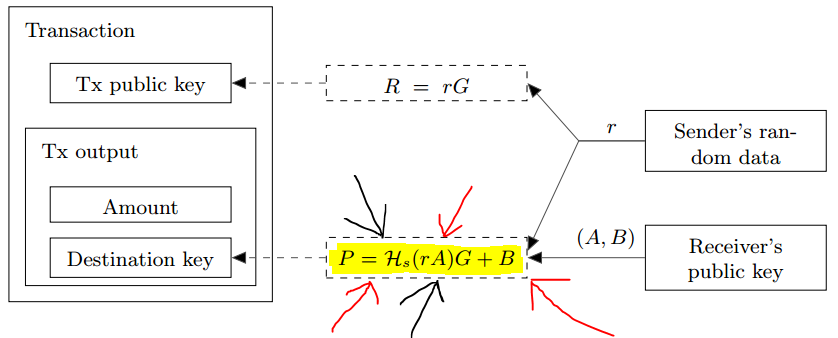
\includegraphics[width=0.8\linewidth]{./images/blog-series/xmr-crypto-luigi1111/stealth-address-cryptenote.png}
\end{figure}

As I've helpfully highlighted and pointed out here, we're looking at \(P = H_s(rA)\cdot G + B\).\par

\textbf{Dual-key} simple refers to the pairs of spend/view keys, which allows ``decoding'' (or removing the unlinkability if you will) stealth addresses \textit{without simultaneously allowing them to be spent}.\par

Now, ignore all that. Let's back up.\par

Alice wants to send a payment to Bob. Alice's \textbf{private spend key} is \(z\), and her \textbf{private view key} is \textbf{y}. Her public address is then \((Z, Y)\) in holy whitepaper order. I've helpfully used letters that aren't referenced above, because \emph{Alice's keys aren't used at all}.\par

Bob's \textbf{public address} is \((A, B)\). Remember from the previous article that the whitepaper helpfully uses \(A\) as the public view key and \(B\) as the public spend key. Presumably Bob's \textbf{private keys} would be \((a, b)\), but Alice (our current perspective) doesn't know them.\par

The final piece needed before ``building'' our first stealth address is \(r\) and \(R\). \(r\) is a new random scalar chosen by Alice for the express purpose of creating a stealth address for Bob. \(R\) is the corresponding curve point for \(rG\). \(r\) is not given to anyone and may be destroyed after use, unless Alice wants to later prove to a 3rd party that she paid Bob. \(R\), however, is added to the transaction for everyone to see. A new \(r\) should be chosen for every single transaction (reusing r to send to the same recipient would result in a stealth address collision!).\par

Here is an example of R at chainradar.com:
\begin{figure}[H]
	\centering
	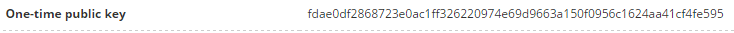
\includegraphics[width=0.8\linewidth]{./images/blog-series/xmr-crypto-luigi1111/R-from-chainradar.png}
\end{figure}

Now that we have our key definitions out of the way, let's create a stealth address! I think walking through the process is the easiest way to understand.\par

\[
	\mathbf{P = H_s(rA)\cdot G+B}
\]

Referenced above we have:
	\begin{enumerate}
		\item \(P\) -- the final \textbf{stealth address} (one-time output key, the destination where funds will actually be sent);
		\item \(H_s\)* -- a \href{https://en.wikipedia.org/wiki/Cryptographic_hash_function}{hashing algorithm} that returns a scalar (i.e., the hash output is interpreted as an integer and reduced modulo \(l\));
		\item \(r\) -- the new random scalar Alice chose for this transaction;
		\item \(A\) -- Bob's \textbf{public view key};
		\item \(G\) -- the standard Ed25519 base point;
		\item \(B\) -- Bob's \textbf{public spend key}.
	\end{enumerate}

	[*Note: the hashing algorithm of choice for Monero and other Cryptonote coins is \href{https://en.wikipedia.org/w/index.php?title=SHA-3&diff=674814400&oldid=674650199#Examples_of_SHA-3_and_Keccak_variants}{keccak-256}. This article's focus is not on hashing algorithms, so if you want to learn more about them please see the linked article. Wikipedia, however, has a good short list of the properties we want:

	\begin{enumerate}
		\item it is quick to compute the hash value for any given message
		\item it is \href{https://en.wikipedia.org/wiki/Computational_complexity_theory#Intractability}{infeasible} to generate a message from its hash value except by trying all possible messages
		\item a small change to a message should change the hash value so extensively that the new hash value appears \textbf{uncorrelated} with the old hash value
		\item it is infeasible to find two different messages with the same hash value
	\end{enumerate}
	\#1 is obvious. \#2 is the one-way property. \#3 is very interesting, as ``uncorrelated'' is quite similar to our magic word, \textbf{unlinkable}. \#4, collision resistance, is very important because a bad algorithm could significantly ``improve'' the chance of a stealth address collision (versus the \(2^{126}\) discussed above).\par

I would add to this list:
	\begin{enumerate}
		\item any length input;
		\item fixed-length output;
		\item output cannot be predicted or chosen in advance (preimage-resistance) -- this is related to \#2 above.]
	\end{enumerate}
Whew, that got long.

\subsubsection{Alright, so let's actually create a stealth address!}
	\begin{enumerate}
		\item Alice does ECDH with her randomly-chosen r and Bob's public view key, \(A\). Let's call this point \textbf{D}. No one other than Alice or Bob can compute \textbf{D} (see the discussion above on ECDH).
		\item Alice uses \(D\) to generate a new scalar; we'll call it \(f\). \(f = H_s(D)\). Yes I like naming things. This is the step that actually \textbf{causes unlinkability} between Bob's outputs (remember \#3 above -- more on this later)!
		\item Alice computes \(F = fG\).
		\item Alice computes \(P = F + B\) (Bob's public spend key).
		\item \(P\) is the stealth destination!
	\end{enumerate}
\subsubsection{Now let's look at Bob's perspective:}
	\begin{enumerate}
		\item Bob receives a transaction; he wants to check if it belongs to him.
		\item Bob retrieves \(R\), which Alice has helpfully attached to the transaction.
		\item Bob computes \(D'\). Note Bob doesn't (yet) know if \(D'\) is equal to \(D\). \(D' = aR\).
		\item Bob computes \(f' = H_s(D')\).
		\item Bob computes \(F' = f'G\).
		\item Bob computes \(P' = F' + B\).
		\item Bob checks if \(P'\) is equal to \(P\), which was included in the transaction as the destination. If yes, Bob realizes he's been paid and does some additional steps (below). If no, Bob ignores the transaction.
	\end{enumerate}
\subsubsection{Some notes:}
	\begin{enumerate}
		\item Computing \(D\) and \(D'\) requires secret data: either \(r\) (Alice) or \(a\) (Bob). Thus, external observers are prevented from proceeding past Alice's step 1. Furthermore, because \(r\) is randomly chosen, even if the observer suspects Alice is sending to Bob's public address (which the observer knows), due to the ECDLP they still can't link this address to \(P\) without knowledge of \(r\) or \(a\) (or pedantically the later steps' values, namely \(D\) and \(f\)).
		\item You may have noticed that this scheme only gives Alice one output for Bob per \(r\), but with auto-denomination Monero and other Cryptonote coins have many outputs per transaction. To get different stealth addresses for each output, Alice (and Bob) append an ``output index'' (an output's position in the transaction: 0, 1, 2, etc.) to \(D\) before hashing it to create the secret shared scalar f. This is a bit of a clarification to Alice's step 2 on \textbf{unlinkability}. That is, while the shared secret \(D\) is already unlinkable to observers, appending an output index allows ``unlimited'' additional unlinkable outputs to be created from one shared secret (see point 3 in the hash section).
		\item Back to the \textbf{dual-key} concept, Bob (or someone working on his behalf with knowledge of \(a\) and \(B\)) can ``scan'' for and detect/link outputs without knowledge of \(b\), which is required below to actually spend that output. The whitepaper calls \((a,B)\) the ``tracking key''.
		\item It is possible to do a non-dual-key stealth addressing scheme, but you must make one of two trade-offs. You can either: 
			\begin{itemize}
				\item use the concept in the whitepaper called a \textbf{truncated address}, which means the view key pair is publicly known and all incoming transactions can be linked (\(a = Hs(B)\)); or 
				\item forego a view key pair entirely, which means scanning requires spending ability (\(P = Hs(rB)\cdot G + B)\)).
			\end{itemize}
	\end{enumerate}
\subsubsection{Bob's Additional Steps}
So, Bob has determined some outputs in a transaction belong to him. Now what does he do? I can imagine two things he \emph{wants} to do: check if this output has already been spent, and (later) actually spend the output. To do either of these things, Bob must first compute the secret key associated with that output (the one-time secret key, \(x\)).
	\begin{enumerate}
		\item Bob recomputes \(f' = Hs(D')\) (as above).
		\item Bob derives \(x = f' + b\) (\(b\) is Bob's private spend key). The ``neat'' thing is that \(P = xG\)! Adding scalars (or points) together preserves linearity. \(P = xG = (f' + b)\cdot G = F' + B\)
		\item To check if \(P\) is spent, Bob computes its ``key image'' and queries the blockchain to see if it is marked as spent. Key image \(I = xH_p(P)\). This will be better explained in the ring signature article. \emph{Fear not!}
		\item To spend \(P\), Bob needs to sign a new transaction with \(x\) (also detailed in the ring signature article).
	\end{enumerate}

	\textbf{[Skip the next section if you hate fun.]}
\subsection{FUN}
\textbf{Now, let's do a ``fun'' exercise with real values for illustration.} \emph{Great...}\par

I'll be using functions that are available in Javascript \href{https://xmr.llcoins.net/}{here}. Doing so allows the curious and discerning reader (\textit{that's you, presumably}) to easily reproduce the results with only a web browser. If you go to the link above and open your browser's console (right-click the page->Inspect, then Console tab), you can enter or copy/paste all the commands below to ``see it in action''. All letters and step numbers match those  above. The scalars b and r below were randomly generated with \code{random_scalar()}; (you obviously can't randomly generate your own if you want to reproduce my results!). You can see the contents of a variable by just typing its name and pressing . ``//'' is a comment in Javascript.\par

Here is the Chrome console:
\begin{figure}[H]
	\centering
	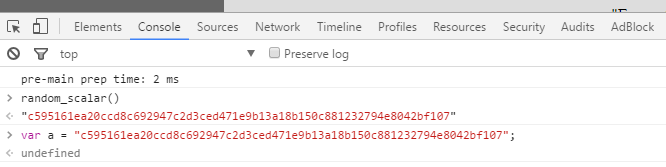
\includegraphics[width=0.8\linewidth]{./images/blog-series/xmr-crypto-luigi1111/stealth-address-chrome-console.png}
\end{figure}

\subsubsection{Preliminary}
\begin{lstlisting}
//Bob's private spend key
 var b = "c595161ea20ccd8c692947c2d3ced471e9b13a18b150c881232794e8042bf107"; 

//Bob's private view key (deterministic derivation); 
//a = "fadf3558b700b88936113be1e5342245bd68a6b1deeb496000c4148ad4b61f02"
var a = hash_to_scalar(b); 

//Bob's public spend key, this function multiplies base G by its input; 
//B = "3bcb82eecc13739b463b386fc1ed991386a046b478bf4864673ca0a229c3cec1"
var B = sec_key_to_pub(b); 

//Bob's public view key; 
//A = "6bb8297dc3b54407ac78ffa4efa4afbe5f1806e5e41aa56ae98c2fe53032bb4b"
var A = sec_key_to_pub(a); 

//returns Bob's public address (for curiosity only), 
//"43tXwm6UNNvSyMdHU4Jfeg4GRgU7KEVAfHo3B5RrXYMjZMRaowr68y12HSo14wv2qcYqqpG1U5AHrJtBdFHKPDE A9UxK6Hy"
pubkeys_to_string(B,A); 

var r = "c91ae3053f640fcad393fb6c74ad9f064c25314c8993c5545306154e070b1f0f";

//R = "396fc23bc389046b214087a9522c0fbd673d2f3f00ab9768f35fa52f953fef22"
var R = sec_key_to_pub(r); 
\end{lstlisting}
\subsubsection{Alice}
\begin{lstlisting}
//ECDH, rA; D = "a1d198629fadc698b48f33dc2e280301679ab2c75a76974fd185ba66ab8418cc"
var D = generate_key_derivation(\(A\), r); 

//0 is the output index; the standard method combines these last few steps into one, but I split them for clarity; 
// f = "bf1d230a09bfdb0bc7fe04cddf8c1635d0ebaaf159ef85dc408ae60879752509"
var f = derivation_to_scalar(D, 0); 

//F = "3e4b39c5b5110d6fbdb77fbcd203709c19fefd28c982a86bda3f3d35fc099738"
var F = sec_key_to_pub(f); 

//``ge'' means group element; this function adds two points together. 
//P = "6cabaac48d3b9043525a703e9e5feb72132f69ea6deca9b4acf9228beb74cd8f"
var P = ge_add(F,B); 
\end{lstlisting}
\subsubsection{Bob}
\begin{lstlisting}
N/A
N/A
var D1 = generate_key_derivation(R, a); //D1 = same as above!
var f1 = derivation_to_scalar(D1, 0); //f1 = same as above!
var F1 = sec_key_to_pub(f1); //F1 = same as above!
var P1 = ge_add(F1,B); //P1 = same as above!
\end{lstlisting}
\subsubsection{Bob's additional steps}
\begin{lstlisting}
N/A

//"sc" means scalar; this function adds two scalars together. 
// x = "97df43cb906896405a8b54ecd4610c92b99de5090b404e5e64b17af17da01601". Now for fun enter sec_key_to_pub(x); and compare with P.
var x = sc_add(f1,b); 

//This combines "hash_to_ec" (Hp, hash to a curve point) and a scalar multiplication of that new point by x. 
// I = "2ba7ee37314d4a1edbeef727f49099c79d55797570cb1206ee2685c94b6550b1" 
// For fun -- spent status
var I = generate_key_image_2(P, x);9 
N/A
\end{lstlisting}
Whew!

\textbf{[End skip.]}
\begin{figure}[H]
	\centering
	
\includegraphics[width=0.8\linewidth]{./images/blog-series/xmr-crypto-luigi1111/tired-dog.jpg}
\end{figure}
tl;dr (\emph{You get one this time!}), stealth addressing allows senders to create ``unlimited'' one-time destination addresses on behalf of the recipient (without any interaction). They can only be recovered and spent by the recipient and can't be publicly linked to each other or the standard address from which they were derived.\par

Until next time!

\section{Borromean Ring Signature原理}
	By Hao Xu.
\subsection{签名}
假设签名者Alice有一个公钥的集合$\{P_{i,j}|0 \leq i \leq n-1 , 0 \leq j \leq m_i-1\}$。其中$n$是环的个数,$m_i$是第\(i\)个环的元素个数。Alice希望用\(n\)个key $\{P_{i,a_i}\}$对应的私钥$x_i$去产生一个环签名,其中$a_i$由Alice挑选,作为环的起点,验证者并不知道。\par
Alice签名步骤如下:
\begin{enumerate}
	\item 对消息\(m\)进行哈希得到\(M\),并统计所有公钥。
	\item 对于每一个$0 \leq i \leq n-1$,
	\begin{enumerate}
		\item 随机选择一个标量$k_i$.
		\item 设置$e_{i,a_i+1}=H(M||k_iG||i||a_i)$.
		\item 对于每个$a_i+1 \leq j < m_i-1$,随机选取$s_{i,j}$的值,并计算
		\begin{equation*}
		e_{i,j+1}=H(M||s_{i,j}G-e_{i,j}P_{i,j}||i||j).
		\end{equation*}
	\end{enumerate}\par
	至此计算了每个环中编号大于$a_i$的所有点的\(e\)值和\(s\)值。
\item 对于每个环,选取编号最大的点的\(s\)和\(e\)值,分别为$s_{i,m_i-1}$和$e_{i,m_i-1}$。并计算$e_0$,公式如下:
\begin{equation*}
e_0=H(s_{0,m_0-1}G-e_{0,m_0-1}P_{0,0}||\dots||s_{n-1,m_{n-1}-1}G-e_{n-1,m_{n-1}-1}P_{n-1,m_{n-1}-1})
\end{equation*}\par 
由公式可知,$e_0$值取决于\(n\)个点的\(s\)和\(e\)的值。
\item 对每个$0 \leq i \leq n-1$:
\begin{enumerate}
	\item 对于每一个$0 \leq j < a_i-1 $,随机选择$s_{i,j}$的值,并计算
			\begin{equation*}
				e_{i,j+1}=H(M||s_{i,j}G-e_{i,j}P_{i,j}||i||j).
			\end{equation*}
			其中$e_{i,0}$即为$e_0$。这一步计算了每个环中编号小于$a_i$的所有点的\(e\)值和\(s\)值,以及$a_i$的\(e\)值。
		\item 计算$a_i$的\(s\)值如下:$s_{i,a_i}=k_i+x_ie_{i,a_i}$.
\end{enumerate}
\end{enumerate}\par 
最后生成的环签名如下:
\begin{equation*}
\sigma =\{e_0, s_{i,j} :0 \leq i \leq n, 0 \leq j \leq m_i\}
\end{equation*}

\subsection{验签}
假设验证者的已知信息为消息\(m\),公钥集$\{P_{i,j}|0 \leq i \leq n-1 , 0 \leq j \leq m_i-1\}$和签名$\sigma$。\par 
验证者验证签名过程如下:\par 
\begin{enumerate}
	\item 对消息\(m\)进行哈希得到\(M\).
	\item 对于每个$0 \leq i \leq n-1$和$0 \leq j \leq m_j-1$,计算$R_{i,j+1}=s_{i,j}G+e_{i,j}P_{i,j}$和$e_{i,j+1}=H(M||R_{i,j+1}||i||j)$.
	\item 计算$e'_0=H(R_{0,m_0-1}||\dots||R_{n-1,m_{n-1}-1})$。并比较$e'_0 \overset{?}{=}e_0$,若相等,则验证通过。
\end{enumerate}
以上签名过程的示意图如\figurename~\ref{fig-borromean-sig}.
\begin{figure}[!htbp]
	\centering
	\begin{tikzpicture}[auto,bend angle=45,node distance=3cm,
		place/.style={circle,draw},marrow/.style={->,very thick}]
		\node[place] (e0) {\(e_0\)};
		\node[place] (e1) [above right of=e0] {\(e_1\)};
		\node[place] (e2) [below right of=e0] {\(e_2\)};
		\node[place] (e3) [above left of=e0] {\(e_3\)};
		\node[place] (e4) [below left of=e0] {\(e_4\)};

		% connection
		\draw [marrow] (e0) to node [swap] {\( (s_0,P_0)\)} (e1);
		\draw [marrow,dashed,red] (e1) to [bend left] node {\( (s_1,P_1)\)} (e2);
		\draw [marrow] (e2) to node  [swap]{\( (s_2,P_2)\)} (e0);

		\draw [marrow] (e0) to node {\( (s_0',P_0')\)} (e3);
		\draw [marrow,dashed,red] (e3) to [bend right] node {\( (s_3,P_3)\)} (e4);
		\draw [marrow] (e4) to node {\( (s_4,P_4)\)} (e0);
	\end{tikzpicture}
	\caption{A Borromean ring signature for \( (P_0|P_1|P_2)\&(P_0'|P_3|P_4)\)}\label{fig-borromean-sig}
\end{figure}

\section{Mix-ins Construction}
	By Xiangmin Li on July 30th, 2017.
\subsection{Notations}
	\begin{itemize}
		\item \(n\): number of mix-in requested 
		\item \(pk_i\):  public keys of the output indexed by the global output index \(i\) 
		\item \(C_i\):  commitment of the output indexed by the global output index \(i\)
		\item \(unlocked\): means the outputs are available for spending 
		\item \(x\): the number of RCT outputs, including those spent. Hence, it's also the upper index limit of global indices of these outputs 
		\item \(y\): the number of unlocked RCT outputs among all RCT ones, including those spent. Hence, it’s also the upper index limit of global indices of these unlocked outputs 
		\item \(z\): the number of recent RCT outputs among \(y\) unlocked ones. Hence, the range of indices for recent RCT outputs should be \([y−z,y]\)
		\item \(\Delta w_c\):  a time window of recent cut off, i.e., the time interval of interest is \([t-\Delta w_c, t]\) given \(t\) is a referenced moment 
		\item \(\Delta w_1\): the unlocked time window for money \
		\item \(\Delta w_2\): the default spendable age of the transaction 
		\item \(\pi\):  the global index of the real output
	\end{itemize}
\subsection{About the global output index}
Similar to the CryptoNote protocol, outputs in Monero are organized into \textcolor{red}{groups} according to their amounts, and a \textcolor{red}{global output index} represents the index of a given output in its corresponding group. This reduces the size of the ring signature by only storing those indices of outputs in the signature instead of the actual public keys.\par
After the activation of RingCT, the denomination of outputs is no longer necessary, and all the RingCT outputs (whose amounts are hidden) are stored in the same group (associated with the amount of 0 XMR by convention). There are 1491097 RingCT outputs as of now, and this transaction generated the two latest outputs at indices of 1491095 and 1491096.\par
For convenience, all the statement henceforth will only refer to RingCTs.
\subsection{Workflow}
There's no check for double spending in the mix-ins selection procedure. And the detail goes as following sequence diagram as \figurename~\ref{fig-mix-ins-selection}.
\begin{figure}[!htbp]
	\centering
	\begin{tikzpicture}[auto,
		place/.style={rectangle,draw},
		marrow/.style={->,thick}]
		\footnotesize
		\node [place,rounded corners,inner sep=2mm] (wallet) {Wallet};
		\node [place,rounded corners,inner sep=2mm] (daemon) [right=7cm of wallet]  {Daemon};

		\node (output-req-send) [below=of wallet] {};
		\node (output-req-recv) [below=of daemon] {};

		% need to set text width for placing list
		\node [place] (output-req-handling) [below=of output-req-recv,text width=6cm] {
			\footnotesize
			Query database for
			\begin{itemize}
					\setlength\topsep{0em}
					\setlength\itemsep{0em}
				\item \(x\)=\#(outputs) of the same amount
				\item \(y\)=\#(unlocked instances) among \(x\)
				\item \(z\)=\#(recent instances) among \(y\)
			\end{itemize}
		};
		\node (output-req-feedback-recv) at (output-req-send |- output-req-handling) {};
		\node [place] (estimate-request-output-count) [below=of output-req-feedback-recv, text width=9cm] {
			\footnotesize
			Estimate
			\begin{itemize}
				\item \#(requested output)\(=a=(n+1)\cdot 1.5+1+\Delta w_1+\Delta w_2\)
				\item \#(requested recent output)\(=b=0.5a\)
			\end{itemize}
		};
		\node [place] (construct-request-output-indices) [below=of estimate-request-output-count, text width=9cm] {
			\footnotesize
			Construct the requested outputs indices set \(I\)
			\begin{itemize}
				\item If \(y\leq a\), set \(I=\{0,1,\dots,y-1,y-1,\dots,y-1\}\) where \(|I|=a\)
				\item Otherwise 
					\begin{enumerate}
						\item \(I=\{\pi\}\)
						\item Pick another \(b\) unique recent output indices by triangular distribution and add then to \(I\)
						\item Pick another \( (a-b-1)\) unique other outputs by triangular distribution and add them to \(I\)
						\item Sort elements in \(I\) according to their values
					\end{enumerate}
			\end{itemize}
		};
		\node (keys-request-send) [below=of construct-request-output-indices] {};
		\node (keys-request-recv) at (keys-request-send -| output-req-handling) {};
		\node [place] (keys-query) [below=of keys-request-recv,text width=6cm] {
			Query database to find out \(\{(i,pk_i,C_i)\}\) (\textcolor{red}{no double spending check here})
		};
		\node (keys-recv) at (keys-request-send |- keys-query) {};
		\node [place] (chk-real-output) [below=of keys-recv] {Check the existence of the real output};
		\node [place] (pick-mix-ins) [below=of chk-real-output, text width=9cm] {
			Pick randomly \(n\) unique and unlocked instances excluding the real output, and construct the MLSAG using these \( (n+1)\) instances. \textcolor{red}{Note}: The \(pk_i\) corresponding to the spent output may be included but that seems to do little good to the linkability
		};
		\node (wallet-end) [below=of pick-mix-ins] {};
		\node (daemon-end) at (wallet-end -| keys-query) {};

		% horizontal arrows
		\draw [marrow] (output-req-send) to node [align=center] {Request the output histogram satisfying\\ \(unlocked\wedge\Delta w_c=1.8\ day\)} (output-req-recv);
		\draw [marrow] (output-req-handling) to node [swap] {\( (x,y,z)\)} (output-req-feedback-recv);
		\draw [marrow] (keys-request-send) to node {Request all key stuff corresponding to outputs indexed by \(I\)} (keys-request-recv);
		\draw [marrow] (keys-query) to node {Response with \(\{(i,pk_i,C_i)\}\)} (keys-recv);
	
		% vertical arrows
		\draw [marrow] (wallet) to (estimate-request-output-count);
		\draw [marrow] (estimate-request-output-count) to (construct-request-output-indices);
		\draw [marrow] (construct-request-output-indices) to (chk-real-output);
		\draw [marrow] (chk-real-output) to (pick-mix-ins);
		\draw [marrow,dashed] (pick-mix-ins) to (wallet-end);

		\draw [marrow] (daemon) to (output-req-handling);
		\draw [marrow] (output-req-handling) to (keys-query);
		\draw [marrow,dashed] (keys-query) to (daemon-end);
	\end{tikzpicture}
	\caption{Mix-ins selection procedure}\label{fig-mix-ins-selection}
\end{figure}

\section{RCT implementation}
	By Xiangmin Li, at 2017-08-11.
\subsection{Overview}
Let \(m\), \(\{l_j\}_{j=1}^m\) be parameters of the Ring-CT scheme, where
	\begin{itemize}
		\item \(m\) is the number of input coins 
		\item \(\{l_j\}\) is a parameter governing the size of the anonymity set hiding the \(j\)-th input coin \(\calS_j\)
	\end{itemize}
There are 2 kinds of Ring-CT in monero project, called the simple Ring-CT (\(m>1\)) and the full Ring-CT (\(m=1\)), where the full version can only be used in case of one ring. These 2 versions of Ring-CT are detailed in following subsections respectively. \par
\subsection{Simple Ring-CT}
	\begin{description}
		\item[Preparation of the transaction key] Generate a seckey-pubkey pair randomly, \( (r,R=r\cdot G)\) for the transaction to conduct.
		\item[Preparation of the output coins] For each coins 
			\[
				coin_k^{(out)}=\left(P_k^{(out)},cn_k^{(out)}, \Pi_k^{(range)}\right)
			\] 
			to send, compute 
			\begin{itemize}
				\item destination address \(P_k^{(out)}=H_s(r\cdot A_k)\cdot G+B_k\), where \(A_k\) and \(B_k\) are respectively, the public viewing key and public spending key for the targeted payee, and \(H_s\) means hashing its input to a scalar over ed25519.
				\item output commitment \(cn_k^{(out)}=y_k\cdot G+b_k\cdot H\), where \(y_k\) is the amount key and \(b_k\) is the amount
				\item \(\Pi_k^{(range)}\) is range proof for amount \(b_k\)
			\end{itemize}
		\item[Mixing Input Coin with Anonymity Set] Parse the input coins as \(\calS=\{\calS_j=(P_j,cn_j)\}_{j=1}^m\), where \(cn_j=x_j\cdot G+a_j\cdot H\) commits the denomination \(a_j\) of \(\calS_j\). For each \(\calS_j\), choose arbitrary \(l_j-1\) coins as mix-ins, thus forming a coin vector. Shuffle coins in \(j\)-th vector to get the mixed coin set \(M_j=[(P_{j,1},cn_{j,1}),(P_{j,2},cn_{j,2}),\dots,(P_{j,l_j},cn_{j,l_j})]\) arranged as a column vector. 
		\item[Preparation of Ring \(\calL_j\) for \(j=1,\dots,m\).] For each \(j=1,2,\dots,(m-1)\), there is exactly one \(\pi_j\in\{1,2,\dots,l_j\}\) such that one coin \((P_{j,\pi_j},cn_{j,\pi_j})\in M_j\) is \(\calS_j\). Make a pseudo commitment \(cn_j^*=x_j^*\cdot G+a_j\cdot H\) (i.e., a commitment on the same amount as the real input coin \(\calS_j\), which is called \texttt{pseudoOuts} in the codebase). And for \(\calL_m\), make its pseudo commitment as 
		\[
			cn_m^*=x_m^*\cdot G+a_m\cdot H=\left(\sum y_k-\sum_{j=1}^{m-1}x_j^*\right)\cdot G+a_m\cdot H
		\] 
		For \(j=1,2,\dots,m\), parse ring as
		\[
			\calL_j=
			\begin{bmatrix}
				P_{j,1} &P_{j,2} &\cdots &P_{j,l_j} \\
				(cn_{j,1}-cn_j^*) &(cn_{j,2}-cn_j^*) &\cdots &(cn_{j,l_j}-cn_j^*)
			\end{bmatrix}
		\]
		We know the secret key for column \([P_{j,\pi_j}, cn_{j,\pi_j}]^T\) as \([sk_j,(x_j-x_j^*)]^T\)
		\item[Generation of MLSAG] For each \(\calL_j\), create an MLSAG on message 
		\[
			M=H_s\left(H_s(\{\calS_j\}_{j=1}^m, \{P_k^{(out)}\}),\{cn_j^*\}_{j=1}^m,\{cn_k^{(out)}\}\right)
		\] 
		(Other relevant but not so important parameters are left out for brevity here). The output of signing is \((\calSPK_j, I_j)\), where \(\calSPK_j\) is the ring signature on \(\calL_j\) and \(I_j\) is the key image (a.k.a, the serial number) of the input key pair \( (sk_j,P_j=sk_j\cdot G)\). Parse the final signature \(\sigma\) on the ring set \(\{\calL_j\}_{j=1}^m\) as 
		\[
			(\calSPK_1,I_1,cn_1^*,\dots,\calSPK_m,I_m,cn_m^*)
		\]
		The signature \(\sigma\), transaction public key \(R\) together with the set of output amount commitment \(\{cn_k^{(out)}\}\) and their range proof \(\{\Pi_k^{(range)}\}\) forms the proof that the transaction is conducted correctly. The payer encrypts the output amount key \(y_k\) and denomination \(b_k\) with the shared secret key \(ss=H_s(r\cdot A_k)\) as follows
		\[
			\begin{aligned}
				y_k^* &= &\quad y_k+H_s(ss) \\
				b_k^* &= &\quad b_k+H_s(H_s(ss))
			\end{aligned}
		\]
		and put \(\{(y_k^*,b_k^*)\}\) in the transaction.
		\item[Verification] Re-create 
			\[
				\calL_j=
				\begin{bmatrix}
					P_{j,1} &P_{j,2} &\cdots &P_{j,l_j} \\
					(cn_{j,1}-cn_j^*) &(cn_{j,2}-cn_j^*) &\cdots &(cn_{j,l_j}-cn_j^*)
				\end{bmatrix}
			\]
			using \(cn_j^*\). Then invoke the verification algorithm of the MLSAG to verify the \(\calSPK_j\). And the amount commitment is checked as verifying the following equality 
			\[
				\sum cn_k^{(out)}+b_0\cdot H=\sum_{j=1}^m cn_j^*
			\]
			where \(b_0\) is the transaction fee. Also, check double spending and the range proof \(\Pi_k^{(range)}\).
	\end{description}
\subsection{Full Ring-CT}
	\begin{description}
		\item[Preparation of the transaction key] Generate a seckey-pubkey pair randomly, \( (r,R=r\cdot G)\) for the transaction to conduct.
		\item[Preparation of the output coins] For each coins \(coin_k^{(out)}=(P_k^{(out)},cn_k^{(out)}, \Pi_k^{(range)})\) to send, compute 
			\begin{itemize}
				\item destination address \(P_k^{(out)}=H_s(r\cdot A_k)\cdot G+B_k\), where \(A_k\) and \(B_k\) are respectively, the public viewing key and public spending key for the targeted payee
				\item output commitment \(cn_k^{(out)}=y_k\cdot G+b_k\cdot H\), where \(y_k\) is the amount key and \(b_k\) is the amount
				\item \(\Pi_k^{(range)}\) is range proof for amount \(b_k\)
			\end{itemize}
		\item[Mixing Input Coin with Anonymity Set] Parse the only input coin as \(\calS_0=(P,cn)\), where \(cn=x\cdot G+a\cdot H\) commits the denomination \(a\) of \(\calS_0\). Choose arbitrary \( (l-1)\) coins as mix-ins, thus forming a coin vector. Shuffle coins in the vector to get the mixed coin vector \(M_0=[(P_1,cn_1),(P_2,cn_2),\dots,(P_l,cn_l)]\) arranged as a column vector. 
		\item[Preparation of Ring \(\calL_0\)] There is exactly one \(\pi\in{1,2,\dots,l}\) such that one coin \((P_{\pi},cn_{\pi})\in M_0\) is \(\calS_0\). Then parse the ring as
		\[
			\calL_0=
			\begin{bmatrix}
				P_1 &\cdots &P_l \\
				\left(cn_1-b_0H-\sum cn_k^{(out)}\right) &\cdots &\left(cn_l-b_0H-\sum cn_k^{(out)}\right)			
			\end{bmatrix}
		\]
		where \(b_0\) is the transaction fee. We know the secret key for column \([P_{\pi}, cn_{\pi}]^T\) as \([sk,(x-\sum y_k)]^T\)
		\item[Generation of MLSAG] Create an MLSAG on message based on ring \(\calL_0\)
		\[
			M=H_s\left(H_s(\calS_0, \{P_k^{(out)}\}),cn,\{cn_k^{(out)}\}\right)
		\] 
		(Other relevant but not so important parameters are left out for brevity here). The output of signing is \( (\calSPK_0, I_0)\), where \(\calSPK_0\) is the ring signature on \(\calL_0\) and \(I_0\) is the key image (a.k.a, the serial number) of the input key pair \( (sk,P=sk\cdot G)\). Parse the final signature \(\sigma\) on the ring \(\calL_0\) as \( (\calSPK_0,I_0)\).\par
		The signature \(\sigma\), transaction public key \(R\) together with the set of range commitment \(\{cn_k^{(out)}\}\) forms the proof that the transaction is conducted correctly. The payer encrypts the output amount key \(y_k\) and denomination \(b_k\) with the shared secret key \(ss=H_s(r\cdot A_k)\) as follows
		\[
			\begin{aligned}
				y_k^* &= &\quad y_k+H_s(ss) \\
				b_k^* &= &\quad b_k+H_s(H_s(ss))
			\end{aligned}
		\]
		and put \(\{(y_k^*,b_k^*)\}\) in the transaction.
		\item[Verification] Re-create 
			\[
				\calL_0=
				\begin{bmatrix}
					P_1 &\cdots &P_l \\
					\left(cn_1-b_0H-\sum cn_k^{(out)}\right) &\cdots &\left(cn_l-b_0H-\sum cn_k^{(out)}\right)			
				\end{bmatrix}
			\]
			Then invoke the verification algorithm of the MLSAG to verify the \(\calSPK_0\). Also, check double spending and the range proof \(\Pi_k^{(range)}\).
	\end{description}

\section{StackExchange Series}
\subsection{Important contributors to monero project}
	\begin{itemize}
		\item \href{https://github.com/vtnerd}{vtnerd}
	\end{itemize}
\subsection{About Commitment}
	\begin{itemize}
		\item \href{https://monero.stackexchange.com/questions/3638/how-are-outpk-mask-and-amount-fields-created-when-spending-rignct-coinbase-txs/3639#3639}{How are outPk, mask and amount fields created when spending RignCT coinbase txs}
		\item \href{https://monero.stackexchange.com/questions/3348/what-are-3-types-of-ring-ct-transactions}{What are 3 types of Ring CT transactions} answered by \href{https://github.com/vtnerd}{vtnerd}
	\end{itemize}
\fi

\end{document}
